%===============================================================================
% !!DO NOT TOUCH!!

% LATEX TEMPLATE BY EMIL PERSSON
% Layout design: Bo Tonnquist, Baseline Management AB, 2018  
\documentclass[10pt]{projectdoc}

%===============================================================================
% QoL

%===============================================================================
% Add packages here

% Packages
\RequirePackage{comment}
\RequirePackage{subcaption}
\RequirePackage{graphicx}
\usepackage[export]{adjustbox}
\usepackage[nolist,nohyperlinks]{acronym}

%===============================================================================
%===============================================================================
% Define accronyms here

% Universities
\acrodef{udea}[UdeA]{Universidad de Antioquia}
\acrodef{utp}[UTP]{Universidad Tecnológica de Panamá}
\acrodef{mdu}[MDU]{Mälardalens Universitet}
\acrodef{mit}[MIT]{Massachusetts Institute of Technology}

% RoboCup
\acrodef{ssl}[SSL]{Small Size League}

% Management
\acrodef{wbs}[WBS]{work breakdown structure}
\acrodef{bom}[BOM]{bill of materials}

% Software
\acrodef{ros2}[ROS2]{Robot Operating System 2}
\acrodef{ros}[ROS]{Robot Operating System}
\acrodef{ai}[AI]{artificial intelligence}
\acrodef{hil}[HIL]{hardware-in-the-loop}
\acrodef{os}[OS]{operating system}
\acrodef{api}[API]{application programming interface}

% Hardware
\acrodef{cad}[CAD]{computer-aided design}
\acrodef{mcu}[MCU]{micro controller unit}
\acrodef{esc}[ESC]{electronic speed controller}
\acrodef{cpu}[CPU]{central processing unit}
\acrodef{pcb}[PCB]{printed circuit board}
\acrodef{imu}[IMU]{Inertial measurement unit}

% Physics
\acrodef{rpm}[RPM]{rotation per minute}
\acrodef{dps}[dps]{degrees per second}
\acrodef{dc}[DC]{direct current}

%===============================================================================

%===============================================================================

\fancyFoot{© ProjectBase 7.0 Baseline Management AB, 2018}{\today}
% REMOVE ALL AUTOMATIC INDENTS FROM PAPER
\setlength{\parindent}{0pt}
% \usepackage[style=ieee]{biblatex}
% \addbibresource{references.bib}
\title{Project plan}
\projectname{Multi-robot Soccer - RoboCup}
\clientname{Mikael Ekström}
\managername{Mudar Ibrahim}
\begin{document}
\maketitle
\thispagestyle{fancy}
\infotable

% Copy and Paste any table into https://www.tablesgenerator.com/
% File -> From latex code... | Edit the imported table and generate new

%===============================================================================
% Sections

%===============================================================================
\section{Project information}
\label{section:project_information}

% Project
This paper covers the project plan for the the project Multi-robot Soccer - RoboCup. This project is a collaboration with \ac{udea} and \ac{utp}. The project consists of developing both the hardware and the software for one \ac{ssl}-RoboCup division B robot. The project will assume and follow Swedish laws and standards, unless the \ac{ssl}-RoboCup rules explicitly requires otherwise. When neither is available or ambiguous, the project will refer to European laws and standards.
% Contributors
The project team consists of eleven contributors split into a hardware and a software team, see Table.\:\ref{tab:contributors_roles}. 
% Software
The software team was further divided into communication, individual robot behaviour and collective robot behaviour. Collective robot behaviour is tasked with deciding the overarching strategy and tactics for the entire robot team. Individual robot behaviour is charged with finding a suitable way to execute the desired behaviour from the perspective of an individual robot. Communication involves simulation and \ac{ssl} interfacing, as well as peer to peer communication. See Fig.\:\ref{fig:software_structure} for a visual understanding of how the different modules connect.
% Hardware
The hardware team was split into four groups: powertrain \& electronics, sensors \& embedded systems, 3D-\acs{cad} \& body design and mechanical design. Powertrain \& electronics designs and implements the power system for the robot including batteries, motors, \ac{esc} and the dribbler. Sensors \& embedded systems integrates the sensors and processes the data. 3D-\acs{cad} develops the chassis and all 3D modelling requirements. Mechanical design develops the kicker system.

\begin{table}
    \centering
    \resizebox{\columnwidth}{!}{\noindent\begin{tabular}{|c|c|c|} \hline
         \textbf{Name}          & \textbf{Role}                                         & \textbf{Task}                                 \\ \hline
         Viktor Eriksson        & Software developer                                    & Collective robot behaviour                    \\ \hline
         Anton Grusell          & Hardware developer                                    & 3D-\acs{cad} \& Body design                   \\ \hline
         Mudar Ibrahim          & Team leader \& Software developer                     & Communication                                 \\ \hline
         Jacob Johanssson       & Software developer                                    & Collective robot behaviour                    \\ \hline
         Aaiza Aziz Khan        & Software developer                                    & Communication                                 \\ \hline
         Carl Larsson           & Software lead \& Software developer                   & Individual robot behaviour                    \\ \hline
         Johanna Melander       & Hardware developer                                    & Mechanical design                             \\ \hline
         Shruti Puthiya Kunnon  & Software developer                                    & Communication                                 \\ \hline
         Pontus Svensson        & Team leader \& Hardware lead \& Hardware developer    & Power-train \& Electronics                    \\ \hline
         Fredrik Westerbom      & Hardware developer                                    & Sensors \& Hardware communication             \\ \hline
         Emil Åberg             & Software developer                                    & Individual robot behaviour \& Communication   \\ \hline
    \end{tabular}}
    \caption{Project contributors, including their roles and assigned tasks.}
    \label{tab:contributors_roles}
\end{table}

\begin{figure}
    \centering
    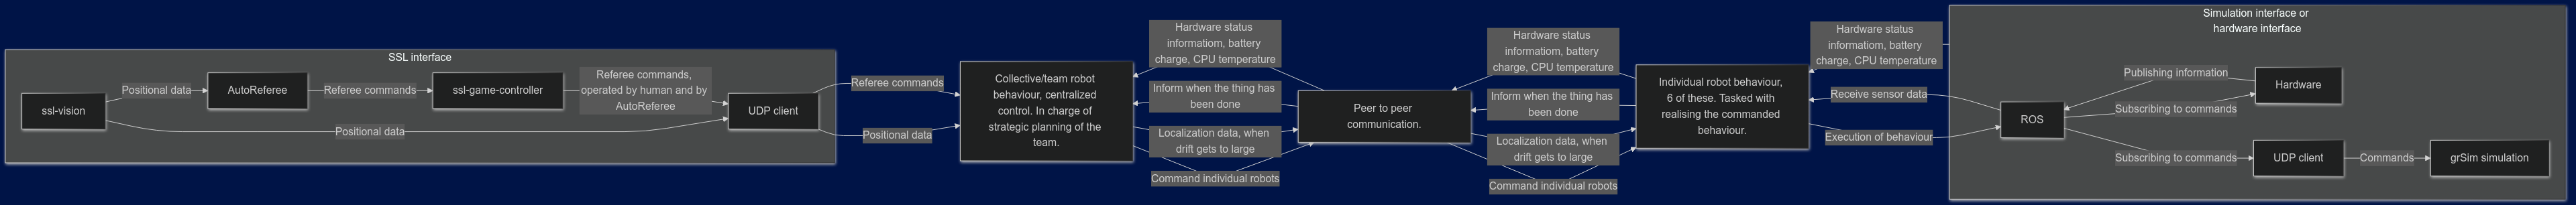
\includegraphics[width=\linewidth]{images/DVA490_software_structure.png}
    \caption{Software structure describing the interaction and connection between the different software modules.}
    \label{fig:software_structure}
\end{figure}

%===============================================================================
%===============================================================================
\section{Executive summary}
\label{section:executive_summary}

This project plan will cover all the necessary information for a sponsor or new member to become integrated with the project, including the standards, methods and tools used. It ensures there is no doubt of what should be delivered, how it should be delivered, how it is to be developed, how it is to be tested and who contributed.

%-------------------------------------------------------------------------------

%\helper{A short summary of the project plan}

%===============================================================================
%===============================================================================
\section{Background}
\label{section:background}

The \ac{ssl}-RoboCup is a tournament where autonomous robots play football\:\cite{da_silva_costa_multi-robot_2024}. There are two different divisions, A and B, with A being the division for more advanced teams\:\cite{noauthor_rules_2024}. Divison A plays on a $12\:\text{m} \times 9\:\text{m}$ field with eleven robots\:\cite{da_silva_costa_multi-robot_2024},\cite{noauthor_rules_2024}. Meanwhile, division B plays with only six robots on a $9\:\text{m} \times 6\:\text{m}$ field\:\cite{da_silva_costa_multi-robot_2024},\cite{noauthor_rules_2024}. 
Each robot needs to be designed to fit inside a cylinder with a diameter of $0.18\:\text{m}$ and a height of $0.15\:\text{m}$\:\cite{noauthor_rules_2024}. The robots are allowed to have both a kicking and a dribbling device\:\cite{noauthor_rules_2024}. The ball used is an orange golf ball which is not allowed to be kicked so that it moves faster than $6.5\:\frac{\text{m}}{\text{s}}$ \cite{noauthor_rules_2024}. 
An \ac{ssl}-RoboCup match consists of first half, half-time break and second half, each one lasting for a period of $300\:\text{s}$\:\cite{noauthor_rules_2024}.

%-------------------------------------------------------------------------------

%\helper{Description with a clear and defined connection to the goals. It is advisable to connect to any related project in the background description.}

%===============================================================================
%===============================================================================
\section{Purpose}
\label{section:purpose}

The purpose of this project is to have a positive impact on both \ac{mdu} and its students. The project would do so in the following ways:
\begin{enumerate}
    \item It would include, and therefore cultivate, international relationships. 
    \item It would help further the multi-robot system research at \ac{mdu}. 
    \item It would contribute to the \ac{ssl}-RoboCup community.
    \item If good performance is obtained (in RoboCup), then it would provide \ac{mdu} with significant institutional branding and recognition.
    \item It would offer fantastic learning opportunities for robotics and embedded system students.
\end{enumerate}

%===============================================================================
%===============================================================================
\section{Goal}
\label{section:goal}

The goal of the project is to deliver the following:
\begin{enumerate}
    \item One \ac{ssl}-RoboCup division B robot which complies with all \ac{ssl}-RoboCup regulations and Swedish laws and standards\footnote{European laws and standards will be deferred to if the Swedish and \ac{ssl}-RoboCup rules, laws and standards are ambiguous or do not address a specific topic.}. The robot is to be capable of:
    \begin{itemize}
        \item Taking actions which are oriented towards goal scoring
        \begin{itemize}
            \item Omnidirectional movement towards target pose
            \item Kick ball
            \item Pass ball
        \end{itemize}
        \item Taking actions which impede the enemy teams ability to score goals
        \begin{itemize}
            \item Block a straight kicked ball from opponents
        \end{itemize}
        \item Not crash into other robots or the arena
        \begin{itemize}
            \item This point is nullified when trying to steal the ball, as long as no permanent damage is inflicted on any robot
        \end{itemize}
        \item Act accordingly to the referee commands and signals
        \item Swap field sides on demand
        \item (See\:\cite{noauthor_rules_2024} for the demands which the robots must fulfil to comply with the \ac{ssl}-RoboCup rules, they will not be listed here but are included as goals)
    \end{itemize}
    \item Simulation interface, allowing for interaction with the simulation software grSim.
    \item Hardware interface, allowing low level control over the robots.
    \item \ac{ssl} interface, allowing for interaction with the \ac{ssl} tools ssl-vision and ssl-game-controller, and integration of AutoReferee.
    \item Robot control using \ac{ros2} Humble and/or micro-\acs{ros}
    \begin{itemize}
        \item Path planning
        \item Setting up robot for a shot
    \end{itemize}
    \item Centralised strategy and tactics planner for the robot team using \ac{ai}, commanding what action each robot should take.
    \item Peer to peer communication protocol using Protobuf and \ac{ros2} Humble, which can select between two carrier frequencies. 
    \item The entire system passing \ac{hil} testing.
\end{enumerate}

%===============================================================================
%===============================================================================
\section{Scope}
\label{section:scope}

The following is part of the scope of the project:
\begin{itemize}
    \item Software
    \begin{itemize}
        \item Simulation interface
        \item Hardware interface
        \item \ac{ssl} interface
        \item Robot control using \ac{ros2} Humble
        \begin{itemize}
            \item Path planning
            \item Enable robot to shot ball towards commanded target
        \end{itemize}
        \item Centralised strategy planner using \ac{ai}
        \item Peer to peer communication using Protobuf and \ac{ros2} Humble
    \end{itemize}
    \item Hardware
    \begin{itemize}
        \item One deployable \ac{ssl}-RoboCup compliant robot adhering to Swedish laws and standards.
        \item Base design
        \item Motor control
        \item Kicker control
    \end{itemize}
\end{itemize}   
Additionally, see the \ac{wbs} available on the project \href{https://github.com/DVA490-474-Project-Course/DVA490_474_PRO1/blob/main/images/WBS.png}{GitHub}\footnote{https://github.com/DVA490-474-Project-Course/DVA490\_474\_PRO1/blob/main/images/WBS.png}.

%-------------------------------------------------------------------------------

%\helper{What is included as part of the project and must be performed in order to deliver the goal. The scope is described with a WBS at the overarching level – main packages with a brief description of each. The complete WBS should be included as an attachment.}

%===============================================================================
%===============================================================================
\section{Limitations}
\label{section:limiations}

The following will not be delivered and thus marks the limitations of the project:
\begin{itemize}
    \item No simulation will be delivered, the already developed grSim will be used.
    \item No global area network will be developed.
    \item Any type of kicks, manoeuvres or similar that was not listed in Goals section\:\ref{section:goal}.
    \item A physical testing environment.
    \item A physical test competition or game.
    \item Benchmarking of physical robots in action.
\end{itemize}
If these were not excluded, they would hamper early development to the point that the delivery of a complete product would be placed at risk.

%-------------------------------------------------------------------------------

%\helper{What the project should not deliver. The purpose is to avoid false expectations among the different stakeholders.}

%===============================================================================
%===============================================================================
\section{Ethical considerations}
\label{section:ethical_considerations}

% Documentation
It is important that everything is openly documented and proper version control is available to ensure transparency, fair play and proof of the true developers. This will be provided by the projects public \href{https://github.com/DVA490-474-Project-Course}{GitHub}\footnote{https://github.com/DVA490-474-Project-Course} page where all code and documentation will be available.
% Sustainability
Proper consideration needs to be taken in regards to the materials used and the disposal of components in the event of replacement or damage. The project will be strict in its disposal and storage of materials and components, following the data sheets and regulations.
% Other fields
Additionally, care must be taken to the possible applications of the research in other fields like warfare and surveillance. The \acs{mit} License will be used to ensure transparency and thus reduce the risk of covert use of the research in unintended ways. 
% Safety and reliability
Finally, proper safety and reliability precautions and practices should be taken to minimise potential damage and harm that the robots can cause. This goes for both damage to robot opponents and disruption of the game, as well as potential harm to humans or the environment. The following precautions and practices will be taken by the project:
\begin{itemize}
    \item Robot status messages will be sent containing information about the status of battery charge and temperatures of microcontroller \acs{cpu}.
    \item Complete stop for a robot if abnormal behaviour is encountered.
    \item Object avoidance
    \item Absolute compliance with data sheets and regulations
\end{itemize}

%===============================================================================
%===============================================================================
\section{Requirement}
\label{section:requirement}

Requirements are necessary to establish in order to ensure that a satisfactory product can be produced and tested, ensuring it meets the original demands placed on the project.

%===============================================================================
\subsection{Product requirements}

The following will describe the features, functionality and specifications which the final product must have.

%-------------------------------------------------------------------------------

%\helper{The product specification describes the product that is to be delivered. It is a description of the product in terms of its functionality, performance, quality, etc.}

%===============================================================================
\subsubsection{Functional requirements}

The following functional requirements were established:
\begin{enumerate}
    \item Robot
    \begin{itemize}
        \item Kick the ball towards designated target
        \item Pass the ball towards designated robot
        \item Block ball
        \item Move to designated target
        \item Omnidiretional (holonomic) movement
        \item Not crash into other robots
        \begin{itemize}
            \item Unless it is an attempt at trying to steal the ball from an opponent or to prevent opponents from scoring a goal
            \item Never acceptable if it causes any permanent damage on either robot
        \end{itemize}
        \item Not crash into the arena
        \item React accordingly to referee signals
        \item Send robot status information
    \end{itemize}
    \item Centralised strategic planner
    \begin{itemize}
        \item \ac{ai} functionality
        \item Switch playing half on demand
        \item Ensure actions for each robot is not taken from an individualistic point of view, but from a overarching team perspective with a strategic plan aimed at obtaining victory
    \end{itemize}
    \item Simulation interface
    \begin{itemize}
        \item Send packages containing robot commands to grSim
    \end{itemize}
    \item Hardware interface
    \begin{itemize}
        \item Control wheel motors
        \item Control kicker
        \item Provide sensor data
        \item Provide robot status information
    \end{itemize}
    \item SSL interface
    \begin{itemize}
        \item Receive positional data from ssl-vision
        \item Receive referee commands from ssl-game-controller
        \begin{itemize}
            \item Have AutoReferee functionality
            \item Have humanly operated referee functionality
        \end{itemize} 
    \end{itemize}
    \item Communication protocol
    \begin{itemize}
        \item Be peer to peer
        \item Ability to select between two carrier frequencies
    \end{itemize}
\end{enumerate}

%-------------------------------------------------------------------------------

%\helper{The functional requirements describe the functions that the product must do.}

%===============================================================================
\subsubsection{Non-functional requirements}

The following non-functional requirements were established:
\begin{enumerate}
    \item Simulate 12 robots.
    \item Comply with all \ac{ssl}-RoboCup rules, see\:\cite{noauthor_rules_2024}.
    \item A latency lower than $400\:\text{ms}$ from any point in time at which the centralised strategy planner gives a command until it starts executing on the robot.
    \item The robot must have four wheels.
    \item The centralised strategy planner must run on a central computer.
    \item Communication protocol
    \begin{itemize}
        \item Use Protobuf
        \item Use \ac{ros2} Humble
    \end{itemize}
\end{enumerate}

%-------------------------------------------------------------------------------

%\helper{The non-functional requirements describe the technical specifications of the product in details: e.g. colors, performance, quality metrics.}

%===============================================================================
\subsection{Project requirements}

The project has locked time and cost, focus will thus be placed on scope to ensure the project does not expand unrealistically, resulting in an inability to deliver the product. The following list describes what must be done in the project to be able to deliver the product:
\begin{itemize}
    \item Limit the project as described in Limitations, see section\:\ref{section:limiations}.
    \item Keep to the scope of the project as described in Scope, see section\:\ref{section:scope}. 
    \item Keep within budget, see Project budget, section\:\ref{section:project_budget}.
    \item Facilitate clear and good communication within the team and with the sponsor.
\end{itemize}

%-------------------------------------------------------------------------------

%\helper{Requirements on the execution and prioritization between the project’s triple constraints.}

%===============================================================================
\subsection{Prerequisites}

The project demands that the sponsors provide the hardware team with full access to the $\text{B.nr}\:326$ workshop and the tools and machines that should be present there. If additional training is required to operate these tools and machines, then the project demands that this training be afforded to the hardware team latest 2024-10-10.

%-------------------------------------------------------------------------------

%\helper{Demands on the project’s sponsor/owner or client that have to be achieved to ensure the project’s execution and result.}

%===============================================================================
%===============================================================================
\section{Situational analysis and stakeholders}
\label{section:situational_analysis_and_stakeholders}

The situational analysis of this RoboCup project involves evaluating both internal and external factors that can impact the project development process. Understanding these important factors gives the team the ability to make accurate and strategical decisions to ensure a successful outcome.  


%===============================================================================
\subsection{SWOT-analysis}
The main reason for this analysis is to identify strengths, weaknesses, opportunities, and threats that stand behind the projects outcome.  This analysis helps the team identify areas of potential growth, manage risks, and capitalise on resources available through partnerships and institutional support. 


\textbf{Strengths:}
\begin{itemize}
    \item Skilled team: the project has well defined team structure with experience in various areas in both software and hardware. 
    \item Strong team collaboration: the team members strive to maintain great relationship with each other.   
    \item Advanced tools and technologies: use of advanced tools and technologies including \ac{ros2}, GoogleTest and tools such as OnShape for 3D-\acs{cad} modelling. 
\end{itemize}

\textbf{Weaknesses:}
\begin{itemize}
    \item Time constraints: the project operates within a fixed timeline, which limits the projects scope and flexibility. 
    \item No time for physical testing: due to the project having a fixed timeline, team members have limited opportunities to test the system in real-world conditions.
    \item Project budget: the project budget is limited and inhibits the teams options. 
    \item Large group experience: the team members lack experience working on a project with a group size this large.
\end{itemize}

\textbf{Opportunities:}
\begin{itemize}
    \item International collaboration: opportunity to add experienced members to the team with \ac{mdu}s international collaboration with \ac{udea} and \ac{utp}, possibly obtaining even greater results. 
    \item Learning and practice: significant potential for students to learn and use advanced technologies. 
\end{itemize}

\textbf{Threats:}
\begin{itemize}
    \item Technical issues: the simulation could differ from reality, which could result in unforeseen implications when deploying the physical system. 
    \item Demands imposed by the stakeholders and sponsors: stakeholders can and may limit the choices available to team members. This could include things like which tools and features are to be used or not used, all of which will affect the quality of project deliverables. 
\end{itemize}

%-------------------------------------------------------------------------------

\begin{comment}
\textbf{Conclusions:}
\begin{itemize}
    \item Need to secure additional funding and focus on continuous skills development
    \item Strategic alliances should be considered to mitigate weaknesses and threats
    \item Constant monitoring and lobbying required to navigate regulatory landscape
\end{itemize}
\end{comment}

%===============================================================================

\subsection{Stakeholder mapping}

Mapping and analysis of individuals, groups, and organisations that might affect or will be affected by the project.

\begin{itemize}
    \item \textbf{Internal Stakeholders:} Mikael Ekström and Emil Persson.
    \item \textbf{Investors:} \ac{mdu} has provided financial support for the project and invested in its success. 
    \item \textbf{Partners:} \ac{udea} and \ac{utp} working with \ac{mdu} on the project.
    \item \textbf{Customers:} Mikael Ekström, the project stakeholder and client, will utilise the autonomous robot once it is completed. 
    \item \textbf{Regulatory Bodies:} RoboCup and Swedish laws set the standards and rules which the project must comply with. 
    \item \textbf{Suppliers:} \ac{mdu} supplies the necessary materials and resources for the project. 
    \item \textbf{Competitors:} Other universities working on RoboCup projects, developing related technologies and solutions. 
\end{itemize}

%===============================================================================
%===============================================================================
\section{Planning}
\label{section:planning}

The project plan is presented in this section.

%===============================================================================
\subsection{Milestone plan}

See Fig.\:\ref{fig:mile_stone} in Appendix\:\ref{appendix:milestone_plan} for the milestone plan.

%-------------------------------------------------------------------------------

%\helper{Stakeholders may want an overarching flow chart or table of the project’s most important milestones as a indicator if the project is falling behind.}

%===============================================================================
\subsection{Work breakdown structure}

The \ac{wbs} is available on the projects \href{https://github.com/DVA490-474-Project-Course/DVA490_474_PRO1/blob/main/images/WBS_updated.png}{GitHub}\footnote{https://github.com/DVA490-474-Project-Course/DVA490\_474\_PRO1/blob/main/images/WBS\_updated.png} page.

%-------------------------------------------------------------------------------

\begin{comment}
The Work Breakdown Structure (WBS) is a fundamental tool in project management, establishing a systematic and structured approach to break down the intricate project into manageable components. This detailed, hierarchical decomposition of the project's scope presents a visual or textual representation that facilitates an understanding of the project's structure, workflow, and tasks necessary for successful project completion. A key note is that the WBS should only include items related to the project and not the project course, this excludes items such as course assignments as they are not a part of the project, only the course.

If you need an anecdote, picture this: "You are a consultant assigned to help clients develop a Work Breakdown Structure (WBS) for their project. This WBS will outline the project's components, giving a clear roadmap of what is to come. You also have internal tasks like time reports, presentations, and assignments for your consulting firm. However, it is important to remember that these internal duties belong outside the client's WBS. They are part of your job, not the client's project. By keeping the WBS client-specific, you maintain clarity and ensure an effective project management strategy."

The WBS dissects the project into multiple layers for ease of management, separating the work into components, work packages, deliverables, and tasks.

\begin{itemize}
\item \textbf{Components} represent the broad sections or stages of the project.
\item \textbf{Work Packages} are subsets of these components, which can be further broken down into specific deliverables.
\item \textbf{Deliverables} are tangible or intangible goods or services produced in the project. They can be handed over physically or digitally to another person or team, forming the backbone of each work package and contributing substantially to the overall project's progression.
\item \textbf{Tasks} represent the smallest work units necessary to complete each deliverable, providing clear action items for project participants.
\end{itemize}

By enabling systematic project planning, effective resource allocation, and reliable progress tracking, the WBS becomes an invaluable aid in navigating the complexity of projects and driving them towards successful outcomes.

A small text-based example, recommend visual based, of applying a WBS for a mobile autonomous robot development project is illustrated below, and only one component is added to keep it short for the example. This example should provide a more tangible understanding of the WBS and its purpose.

\begin{table}[H]
    \centering
    \begin{tabular}{|l|l|l|}
    \hline
    \textbf{\textbf{ID}} & \textbf{Type} & \textbf{Activity}                                          \\ \hline
    1                    & Root          & Mobile Autonomous Robot Development                        \\ \hline
    1.1                  & Component     & Navigation and Path Planning                               \\ \hline
    1.1.1                & Work Package  & Sensor Integration                                         \\ \hline
    1.1.1.1              & Deliverable   & Sensor Selection Report                                    \\ \hline
    1.1.1.1.1            & Task          & Research Suitable Sensors (LiDAR, RADAR, Ultrasonic, etc.) \\ \hline
    1.1.1.1.2            & Task          & Prepare Sensor Selection Report                            \\ \hline
    1.1.1.2              & Deliverable   & Sensor Installation Manual                                 \\ \hline
    1.1.1.2.1            & Task          & Install Sensors on Robot Chassis                           \\ \hline
    1.1.1.2.2            & Task          & Prepare Sensor Installation Manual                         \\ \hline
    1.1.1.3              & Deliverable   & Sensor Data Fusion                                         \\ \hline
    1.1.1.3.1            & Task          & Develop Sensor Data Fusion Algorithm                       \\ \hline
    1.1.1.3.2            & Task          & Implement and Test Sensor Data Fusion Algorithm            \\ \hline
    1.1.2                & Work Package  & Path Planning                                              \\ \hline
    1.1.2.1              & Deliverable   & Path Planning                                              \\ \hline
    1.1.2.1.1            & Task          & Research Suitable Path Planning Algorithms                 \\ \hline
    1.1.2.1.2            & Task          & Implement Selected Path Planning Algorithm                 \\ \hline
    1.1.2.2              & Deliverable   & Path Planning Testing Report                               \\ \hline
    1.1.2.2.1            & Task          & Test Path Planning Algorithm in Simulated Environment      \\ \hline
    1.1.2.2.2            & Task          & Prepare Path Planning Testing Report                       \\ \hline
    \end{tabular}%
\end{table}
\end{comment}

%===============================================================================
\subsection{Schedule}

The project schedule can be seen in Fig.\:\ref{fig:project_schedule}, with software schedule in Fig.\:\ref{fig:software_schedule} and hardware schedule in Fig.\:\ref{fig:hardware_schedule}.

\begin{figure}[H]
    \centering
    \begin{subfigure}[b]{0.55\textwidth}
       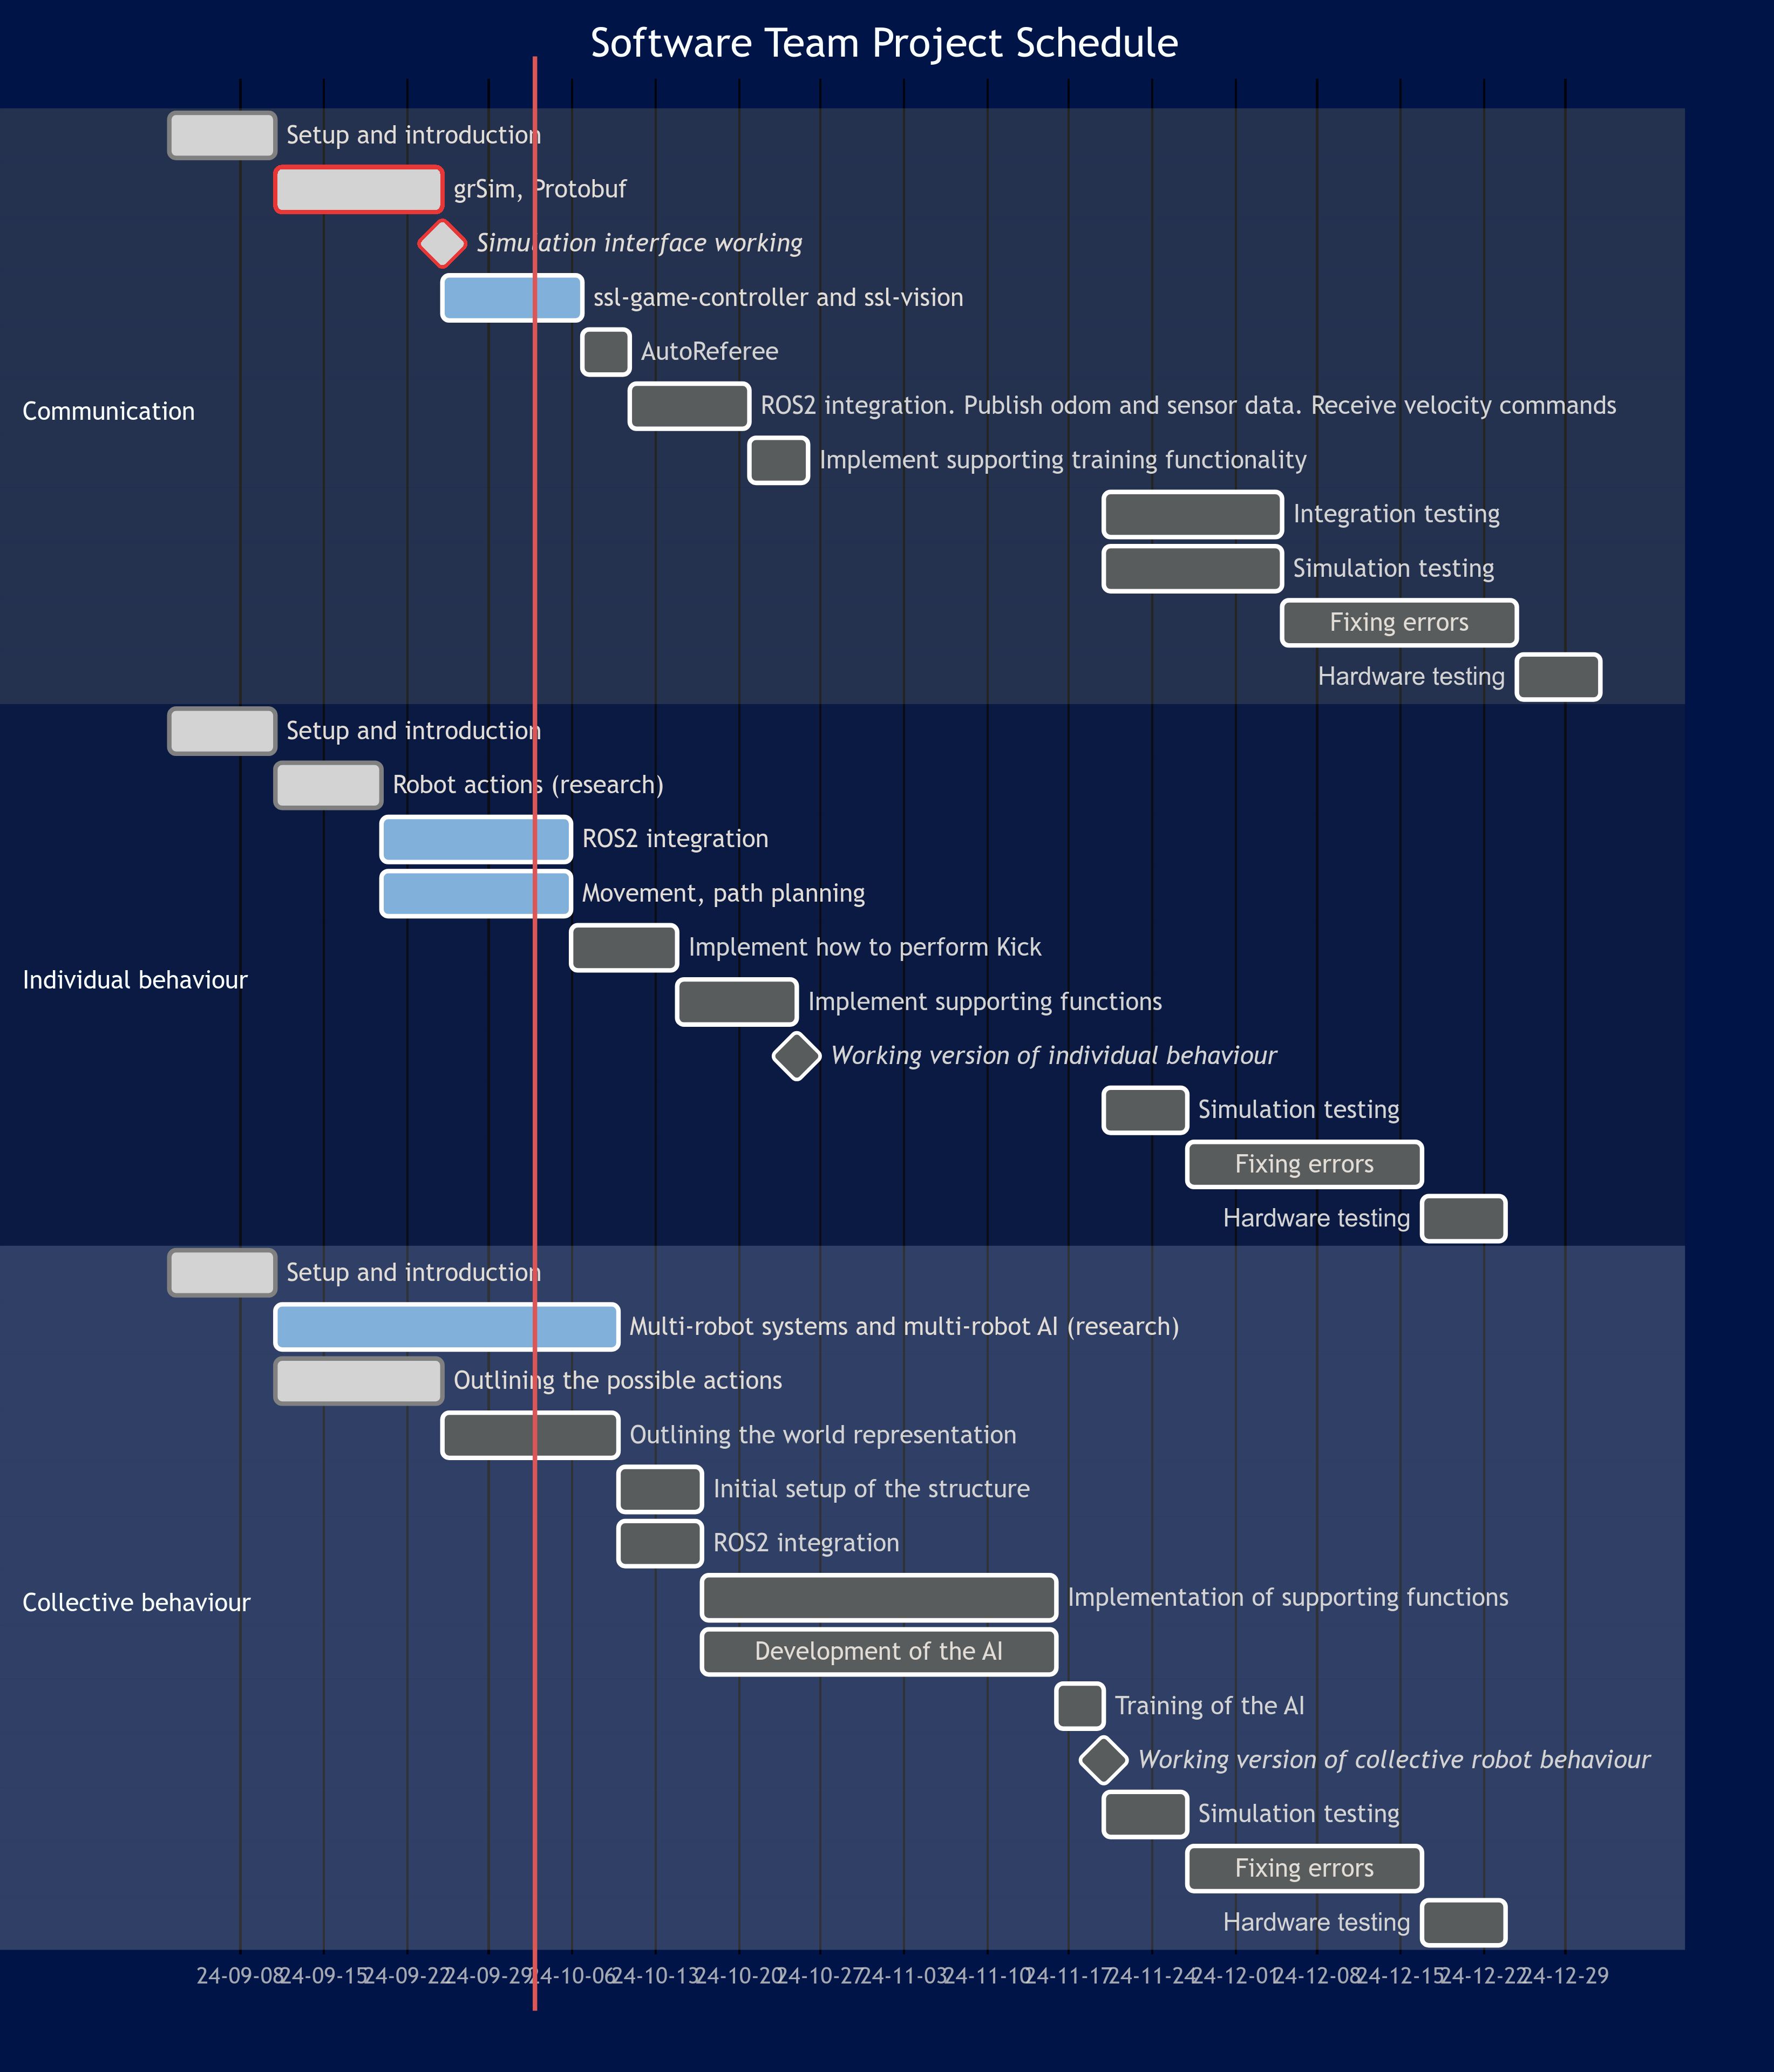
\includegraphics[width=0.95\linewidth]{images/DVA490_software_team_project_schedule.png}
       \caption{Software team schedule.}
       \label{fig:software_schedule} 
    \end{subfigure}
    \hfill
    \begin{subfigure}[b]{0.55\textwidth}
       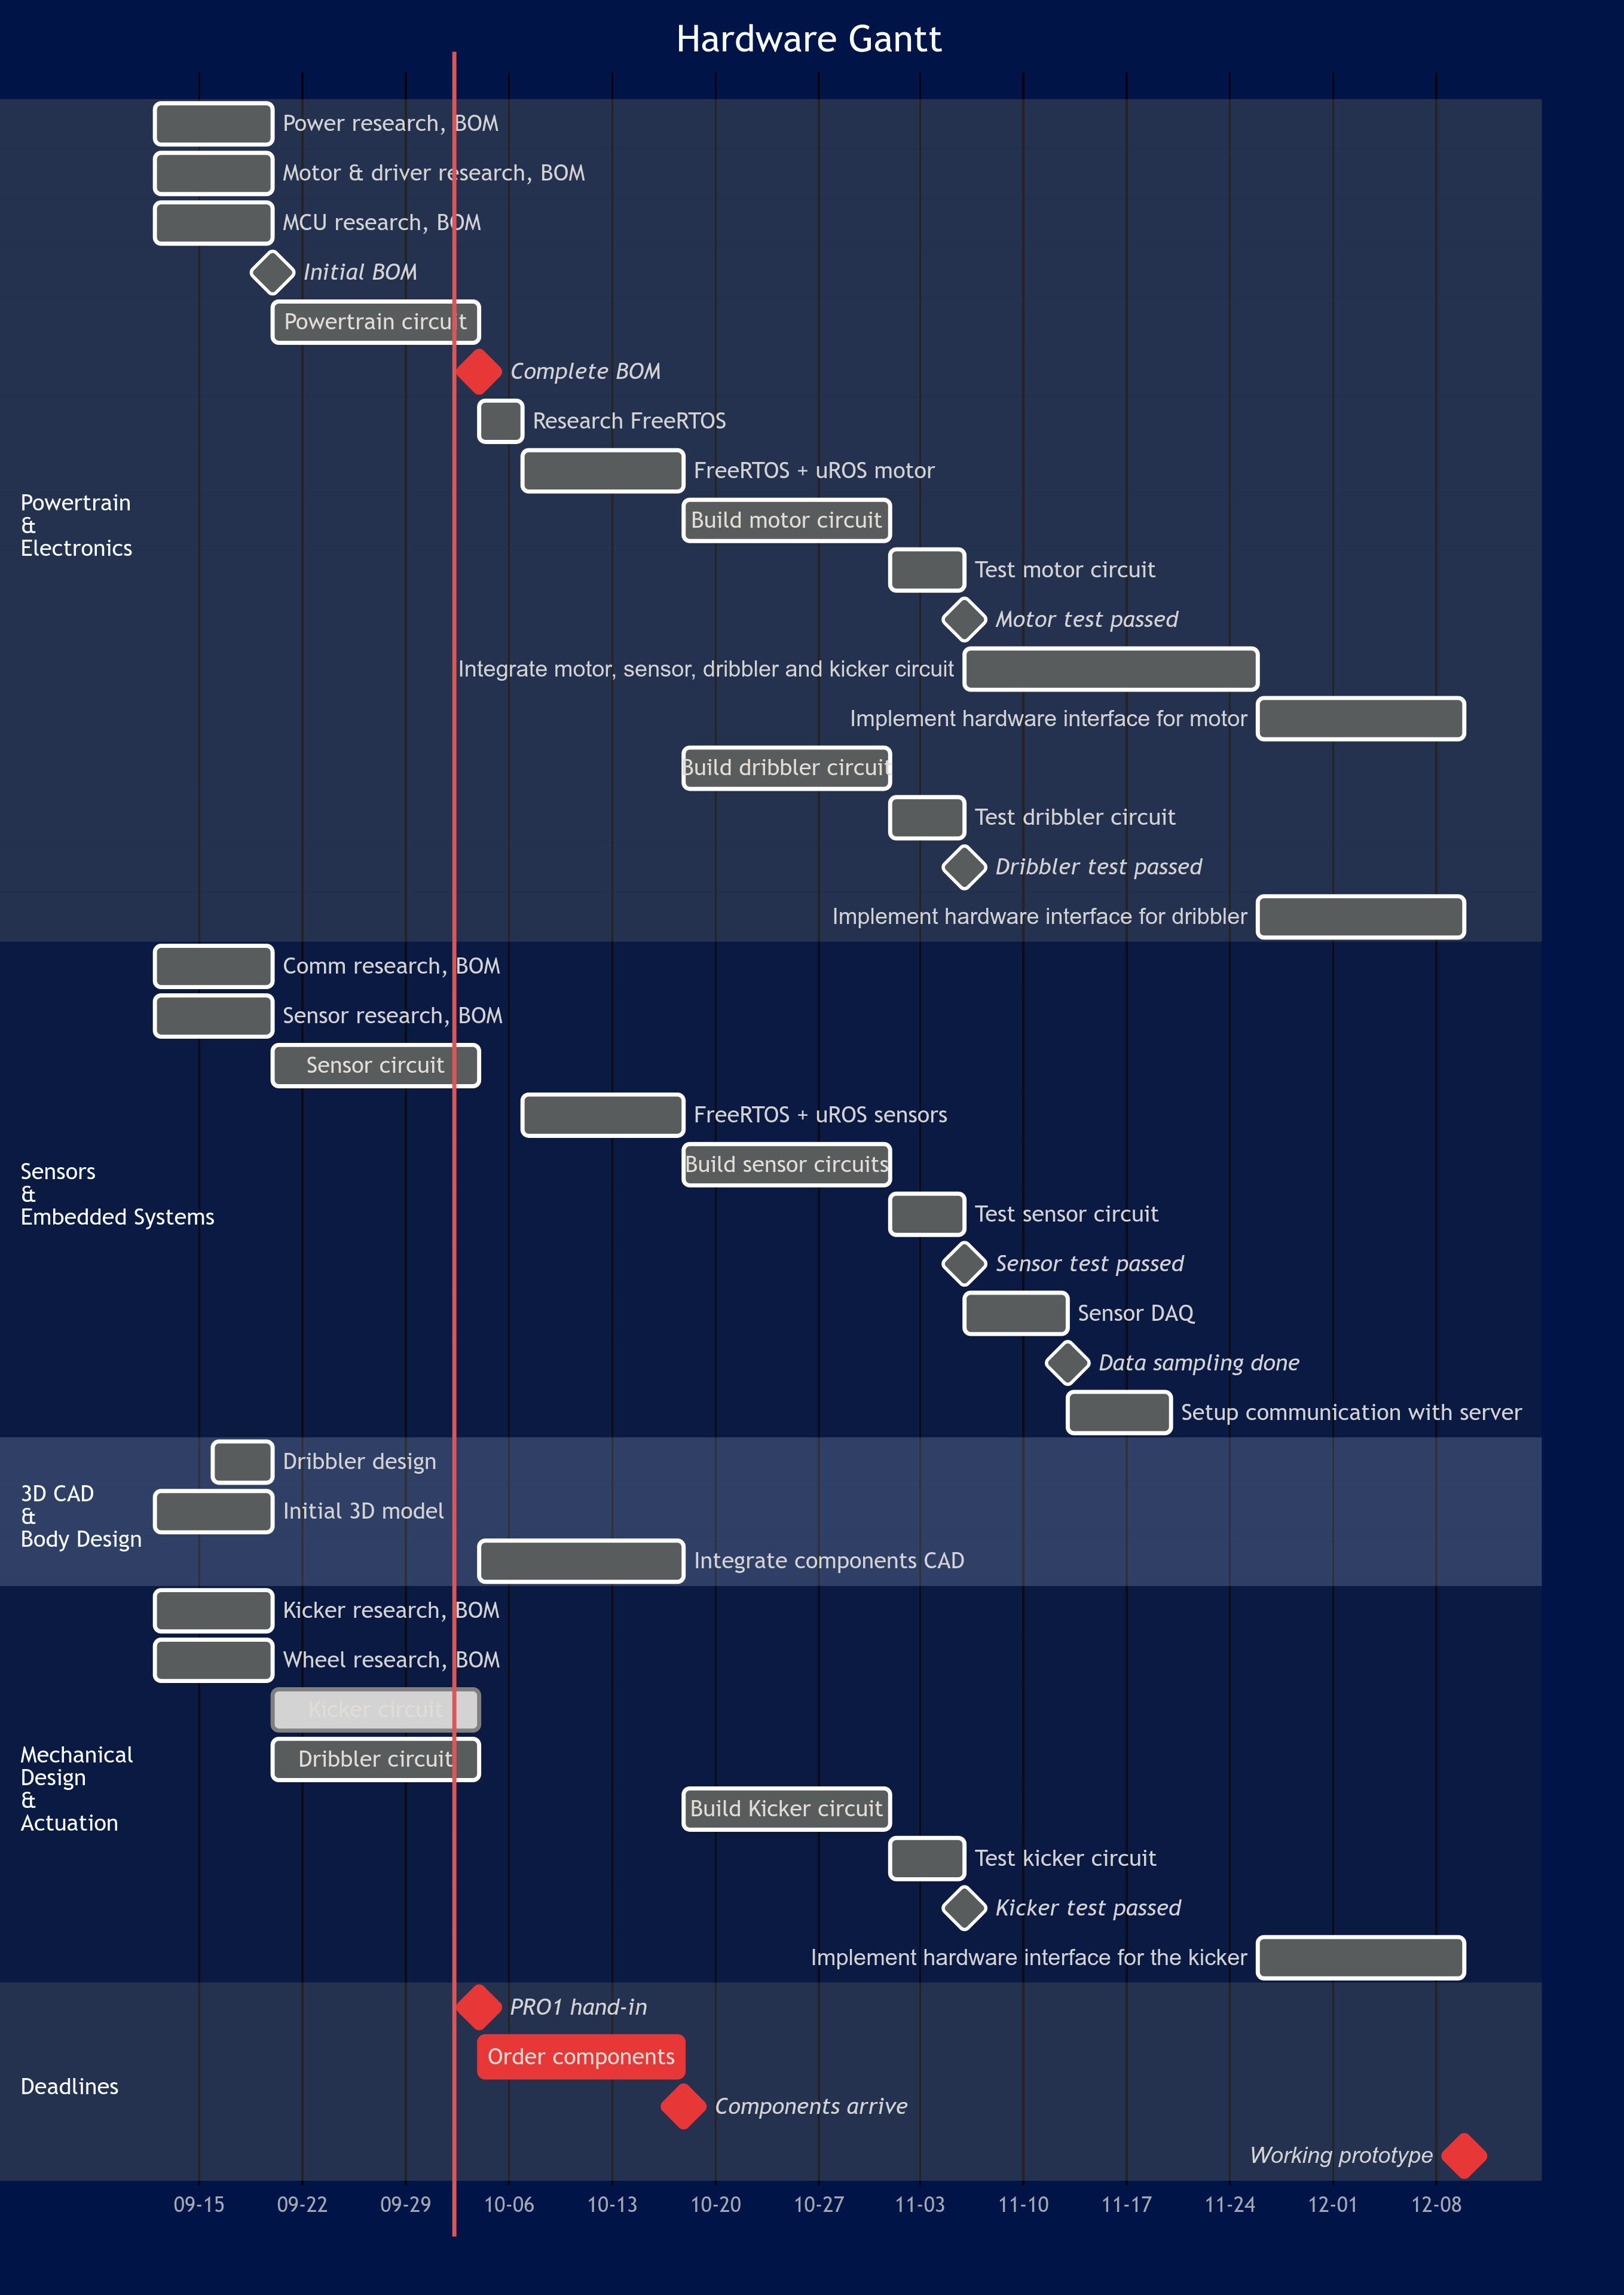
\includegraphics[width=0.95\linewidth]{images/DVA490_hardware_team_project_schedule.png}
       \caption{Hardware team schedule.}
       \label{fig:hardware_schedule}
    \end{subfigure}
    \caption{The project schedule.}
    \label{fig:project_schedule}
\end{figure}

%-------------------------------------------------------------------------------

%\helper{Activity plan with a time axis where duration and connection between activities and milestones are shown.}

%===============================================================================
%===============================================================================
\section{Staffing}
\label{section:staffing}

The staffing plan, in terms of the staff and their roles, were arranged by external sources (sponsor), however tasks were assigned internally based on qualification, collaboration and each team members wishes. The roles and tasks of each project member can be seen in Table.\:\ref{tab:contributors_roles}.

%------------------------------------------------------------------------------

%\helper{Example of a staffing plan, add references to other plans that might include additional information. }

%===============================================================================
\subsection{Roles, responsibilities and authorities}
\label{section:staffing_roles_responsibilities_and_authorities}

%The project teams, and their tasks, have been organised to try to ensure good collaboration, effective use of the members skills and qualifications, as well as their wishes. 
Three authoritative roles with their own responsibilities were assigned (by the sponsor):
\begin{itemize}
    \item Team Leader: Responsible for guiding and coordinating the group to achieve a common goal. A team leader is also responsible for making plans, assigning tasks, ensuring team collaboration, solving conflict, motivating the group and making key decision. One of the main responsibilities of a team leader is to communicate between the team and stakeholders, ensuring that the development process follows the broader project vision.  
    \item Software lead: Organises the software team to ensure work continues smoothly and that the software requirements are met. This includes scheduling, overseeing the software teams progress, planning the software layout and thorough inspection of standards and requirements. 
    \item Hardware lead: Manages the hardware team by overseeing the tasks, provide planning and making sure all requirements are met.
\end{itemize}

%------------------------------------------------------------------------------

\begin{comment}
Our project team structure is specifically crafted to leverage the distinctive skills and capabilities of each team member, fostering effective teamwork. The key roles, responsibilities, and authorities in our project include:

\begin{itemize}
    \item \textbf{Software (SW) Team Lead:} Leads the software team, responsible for overseeing all activities related to software development, ensures that software requirements are met and coordinates with the developers on the software team.
    \item \textbf{Hardware (HW) Team Lead:} Leads the hardware team, responsible for all activities related to hardware development, ensures that hardware requirements are met and coordinates with the developers on the hardware team.
    \item \textbf{Software (SW) Developer:} Implements software components, conducts testing and debugging, and addresses software-related issues.
    \item \textbf{Hardware (HW) Developer:} Designs, tests, and debugs hardware components, addresses hardware-related issues.
\end{itemize}
\end{comment}

%===============================================================================
\subsection{Staffing plan}

The staffing plan is described in Table.\:\ref{tab:contributors_roles}.

%------------------------------------------------------------------------------

\begin{comment}
Our staffing plan assigns roles to each member of our project team as follows:

\begin{itemize}
    \item Stieg Larsson - Software Team Lead
    \item Astrid Lindgren - Hardware Team Lead
    \item Henning Mankell - Software Developer
    \item Selma Lagerlöf - Hardware Developer
\end{itemize}

Each individual was chosen for their role based on their skills, experience, and interest in the project. Regular meetings will be held to ensure that everyone is on track and to address any concerns that may arise.
\end{comment}

%===============================================================================
%===============================================================================
\section{Project budget}
An estimated project budget is shown in Table.\:\ref{tab:estimated_budget}. For a more complete view of the project budget see the preliminary \ac{bom} in Table.\:\ref{tab:bom} available in Appendix\:\ref{appendix:bom}.
\label{section:project_budget}

\begin{table}[H]
    \begin{tabularx}{\columnwidth}{|X|X|X|X|}
        \hline
        Internal costs & External costs & Other costs & Summary \\ \hline
        0              & 20000           & 0           & 20000    \\ \hline
    \end{tabularx}
    \caption{Estimated project budget, all in SEK.}
    \label{tab:estimated_budget}
\end{table}

%-------------------------------------------------------------------------------

\begin{comment}
\helper{The project’s preliminary calculation – a  outline of internal and external costs for resources needed to execute the project.}

\begin{table}[H]
    \begin{tabularx}{\columnwidth}{|X|X|X|X|}
        \hline
        Internal costs & External costs & Other costs & Summary \\ \hline
                       &                &             &         \\ \hline
                       &                &             &         \\ \hline
                       &                &             &         \\ \hline
\end{tabularx}
\end{table}
\end{comment}

%===============================================================================
\newpage
%===============================================================================
\section{Development Plan}
\label{section:development_plan}

This development plan details the development process for the project, and contains important project information. It is crucial to be familiar with all of its details to be able to contribute to the project.

%------------------------------------------------------------------------------

%\helper{Example of a development plan}
%This Development Plan provides a comprehensive roadmap for the project, detailing our technical approach, the development process, the methodologies we employ, and each team member's distinct roles and responsibilities. The plan is designed to facilitate seamless integration for new members joining at any project lifecycle stage. By becoming familiar with the plan, you will gain crucial insights into our work processes and project-related information, enabling you to contribute effectively and align with the team's objectives.

%===============================================================================
\subsection{Development Methodology}

The project team will follow a makeshift model which is akin to the waterfall model because of the time limit placed on the project. This time limit makes it unfeasible for the team to learn a new system, thus defaulting to having a work structure which is similar to the commonly known waterfall model.

%------------------------------------------------------------------------------

% Our team strictly adheres to [specific methodology - e.g., Agile, Scrum, Waterfall, etc.]. We chose this methodology due to its [specific benefits], encompassing practices such as [describe practices].

%===============================================================================
\subsection{Team Structure and Roles}

The team structure and roles are covered in Staffing (see section\:\ref{section:staffing}) and in Table.\:\ref{tab:contributors_roles}.

%------------------------------------------------------------------------------

\begin{comment}
Please note: The roles listed here might have additional responsibilities outlined in the corresponding plans (Documentation Plan, Communication Plan, Testing Plan).

Our team comprises the following roles:

\begin{itemize}
    \item \textbf{Hardware Team Leader:} Manages the hardware development process, coordinates with the software team, and ensures timely delivery while maintaining quality standards.
    \item \textbf{Software Team Leader:} Oversee the software development process, collaborates with the hardware team, and ensure project deadlines are met with high-quality deliverables.
    \item \textbf{Hardware Developer:} Designs, develops, tests, and troubleshoots hardware components and collaborates with the software team.
    \item \textbf{Software Developer:} Develops, tests, and debugs software modules and coordinates with the hardware team.
\end{itemize}
\end{comment}

%===============================================================================
\subsection{Tools, Technologies, and Systems}
\label{subsection:tools_technologies_and_systems}

The \ac{os} that are going to be used are:
\begin{itemize}
    \item \href{https://releases.ubuntu.com/jammy/}{Ubuntu 22.04 LTS}: Ubuntu will be used by all software developers.
    \begin{itemize}
        \item \href{https://kubuntu.org/getkubuntu/}{Kubuntu 22.04.05}: Kubuntu will be used by one software developer.
    \end{itemize}
    \item \href{https://www.microsoft.com/en-us/download/windows}{Microsoft Windows}: Windows will be used by hardware team members for general use. Versions:
    \begin{itemize}
        \item 22H2 (\ac{os} Build 19045.4894)
    \end{itemize}
\end{itemize}

The following software development tools will be used in the project:
\begin{itemize}
    \item \href{https://www.vim.org/vim-8.2-released.php}{Vim}: Vim will be used for coding. Versions:
    \begin{itemize}
        \item 8.2
        \item 8.2.2
    \end{itemize}
    \item \href{https://neovim.io/}{Neovim}: Neovim will be used for coding. Versions:
    \begin{itemize}
        \item 0.10.0
        \item 0.10.1
    \end{itemize}
    \item \href{https://www.sublimetext.com/}{Sublime Text}: Sublime Text will be used for coding. Versions:
    \begin{itemize}
        \item 4180
    \end{itemize}
    \item \href{https://code.visualstudio.com/}{Visual Studio Code}: Visual Studio Code will be used for coding. Versions:
    \begin{itemize}
        \item 1.93.0
        \item 1.93.1
    \end{itemize}
    \item \href{https://www.jetbrains.com/clion/}{CLion}: CLion will be used for coding. Versions:
    \begin{itemize}
        \item 2024.2.2
    \end{itemize}
    \item \href{https://cmake.org/}{CMake version 20}: CMake is the build tool which will be used.
    \item \href{https://github.com/}{GitHub}: GitHub will be used for version control.
    \item \href{https://gitforwindows.org/}{Git Bash}: A terminal with Linux commands for Windows. Used by hardware team members as a replacement for Windows cmd and used for maintaining GitHub repository. Versions:
    \begin{itemize}
        \item 2,46,0,windows,1
    \end{itemize}
\end{itemize}

Code is to be written in the programming languages:
\begin{itemize}
    \item \href{https://en.cppreference.com/w/cpp/20}{C++ standard 20}: all code which is to run on the final system is to be written in C++.
\end{itemize}  

The project will leverage the following libraries, middleware and formats:
\begin{itemize}
    \item \href{https://github.com/RoboCup-SSL/grSim}{grSim}: grSim will be used for all simulation purposes.
    \item \href{https://github.com/RoboCup-SSL/ssl-vision}{ssl-vision}: This tool provides the positional data provided by the cameras present during \ac{ssl}-RoboCup games.
    \item \href{https://github.com/RoboCup-SSL/ssl-game-controller}{ssl-game-controller}: This tool is used by the referee (human operator), during \ac{ssl}-RoboCup games.
    \item \href{https://github.com/TIGERs-Mannheim/AutoReferee}{AutoReferee version 1.4.1}: auto referee software which will run during \ac{ssl}-RoboCup games.
    \item \href{https://docs.ros.org/en/humble/index.html}{\ac{ros2} Humble}: \ac{ros2} Humble is going to be used to control the robots and for communication.
    \item \href{https://docs.nav2.org/index.html}{Nav2}: Nav2 is going to be used for object avoidance and local path planning.
    \item \href{https://github.com/protocolbuffers/protobuf}{Protobuf}: Protobuf will be used for communication and communication interfaces.
    \item \href{https://freertos.org/}{FreeRTOS}: FreeRTOS will be used for low level reliability and threading.
    \item \href{https://google.github.io/googletest/}{GoogleTest}: GoogleTest will be used for software testing.
\end{itemize}

The project will utilise the following hardware tools:
\begin{itemize}
    \item \href{https://www.onshape.com/en/}{OnShape}: OnShape will be used for 3D-\acs{cad} modelling.
    \item \href{https://www.kicad.org/}{KiCAD version 8.0.5}: KiCAD will be used for creating electrical schematics.
    \item \href{}{3D printer}: 3D printer will be used for printing the following components:
    \begin{itemize}
        \item Chassi
        \item Wheels
        \item Motor mounts
        \item Kicker mount
        \item Dribbler mount
    \end{itemize}
    \item \href{}{Soldering station}: Soldering station will be used for soldering the components on \ac{pcb}.
    \item \href{}{Lab bench power supply}: The lab bench power supply will be used for testing the system without a battery.
\end{itemize}

The hardware which will be used:
\begin{itemize}
    \item See Table.\:\ref{tab:bom} available in Appendix\:\ref{appendix:bom}.
\end{itemize}

The project management tools which will be used in the the project are:
\begin{itemize}
    \item \href{https://mermaid.js.org/}{Mermaid}: Mermaid will be used to create gantt charts and block diagrams.
    \item \href{https://www.edrawmax.com/}{EdrawMax}: EdrawMax will be used to create the \ac{wbs}.
    \item \href{https://www.drawio.com/}{draw.io}: draw.io will be used to create the milestone plan.
    \item \href{https://www.microsoft.com/en-us/microsoft-365/excel}{Microsoft Excel}: Excel will be used to create \ac{bom}.
    \item \href{https://www.zotero.org/}{Zotero}: Zotero will be used for reference management.
\end{itemize}

The following communication tools will be used:
\begin{itemize}
    \item \href{https://discord.com/}{Discord}: All team communication is going to take place on discord.
    \item \href{https://www.microsoft.com/en-us/microsoft-365/outlook/email-and-calendar-software-microsoft-outlook}{Outlook}: Outlook will be used for communication with supervisors, stakeholders, additional resources (such as teachers with specific knowledge) and retailers of electronic components and sensors.
    \item \href{https://www.microsoft.com/en-us/microsoft-teams/log-in}{Microsoft Teams}: Teams will be used for communication with collaborators (\ac{udea} and \ac{utp}).
\end{itemize}

%------------------------------------------------------------------------------

\begin{comment}
We leverage the following tools, technologies, and systems in our project:

\begin{itemize}
\item \textbf{Software Development Tools:} Include various programming languages and 3D modelling software. For instance, [Programming Language] is used for [purpose] and can be downloaded from [source]. For 3D modelling, we use [Software name], which can be downloaded from [source].
\item \textbf{Project Management Tools:} We utilize [Tool/Platform Name, version] for [purpose], and it can be downloaded from [source].
\item \textbf{Communication Tools:} For effective communication, we use [Tool/Platform Name, version], which can be downloaded from [source].
\item \textbf{Hardware Tools and Software:} We utilize tools like a 3D printer ([specify model]) and PCB Design Software ([Software Name]) which can be downloaded from [source].
\item \textbf{Operating Systems:} We primarily operate on [Operating System name and version]. Please align your system with the same for consistency and compatibility. If your system operates differently, notify the team for assistance with potential compatibility issues.
\item \textbf{Hardware:} We primarily use [Computer model/brand] with [specify processor, RAM, storage]. Please let us know if you use a different model for compatibility checks.
\end{itemize}

Please install the correct version numbers as specified for consistency and compatibility.
\end{comment}

%===============================================================================
\subsection{Coding Standards and Guidelines}

The project will strictly adhere to the Google C++ Style Guide coding standard and the file structure described in the projects GitHub repository \href{https://github.com/DVA490-474-Project-Course/project-structure}{project-structure}\footnote{https://github.com/DVA490-474-Project-Course/project-structure}. This was done to ensure uniformity, facilitate future development and allow for easy contribution. 

%------------------------------------------------------------------------------

%To ensure high code quality and readability, we follow these coding standards and guidelines: [Outline specific standards and guidelines]. For more comprehensive information, refer to our detailed coding standards document [footnote or ref to document].

%===============================================================================
\subsection{Version Control}
\label{subsection:version_control}

The project will use the version control tool Git to manage changes, versions, history and documentation of all files in the project. The projects \href{https://github.com/DVA490-474-Project-Course}{GitHub}\footnote{https://github.com/DVA490-474-Project-Course} page will contain all the project material and is public and available to everyone.

%------------------------------------------------------------------------------

%We utilize [Version Control System Name, e.g., Git] to manage changes to our project files and maintain different versions. For detailed guidance on using this system, please refer to our [footnote or ref to version control usage guide].

%===============================================================================
\subsection{Testing and Quality Assurance}

% Software
Software testing and quality assurance will be done using GoogleTest. Unit tests will be created for every developed function. Integration tests will additionally be created for every module and sub module. All tests are to be run before committing a new feature or change to GitHub.

% Hardware
Standardised tests for the hardware will be used to calibrate sensors and verify that they behave according to the specifications in the data sheet. These tests should be done every time the robot is used. The hardware interface will use GoogleTest for testing and quality assurance. Unit tests will be created for every developed function.

%------------------------------------------------------------------------------

%We employ [describe testing methodologies] for our testing and QA. For detailed information on our testing process, refer to our [footnote or ref to Testing and QA document or section].

%===============================================================================
\subsection{Integration and Deployment}
\label{subsection:integration_and_deployment}

The integration of the system will follow a structured approach, combining both software and hardware modules. 
Each software module will be developed separately and they will be integrated together once they are ready and have passed their individual unit tests for all the functions they contain. Software modules will first be integrated together with other software modules and tested using integration tests. Afterwards, the hardware components will be integrated in the tests, such as the sensors, motors, and kickers. They will be integrated one at a time with a focus on ensuring accurate output and functionality when combined with the software. 

It is very important to always test and verify the functionality of the modules during the integration phase. Verification will be done by performing unit, integration, and \ac{hil} tests. 
The software modules will be tested in a simulation environment using grSim, while \ac{hil} tests will simulate real-world conditions by integrating hardware components. 

Once the functionality of the modules has been verified and all tests have passed, the deployment phase begins. At this point full deployment tests will be done, which consist of testing the entire system in deployment settings ensuring the functionality of the complete system.

%------------------------------------------------------------------------------

%Our integration strategy involves [describe strategy, e.g., Continuous Integration]. The deployment process includes [describe process], facilitated by specific tools. For comprehensive information on these processes, refer to our integration and deployment guide [footnote or ref to guide].

%===============================================================================
\newpage
%===============================================================================
\section{Communication plan}
\label{section:communication_plan}

The communication plan was established to guarantee that the correct target audience receives the necessary information at the right time and through appropriate channels, see Table.\:\ref{tab:communication_plan}.

\begin{table}
    \centering
    \resizebox{\columnwidth}{!}{\noindent\begin{tabular}{|c|c|c|c|c|c|} \hline
         \textbf{Target audience}   & \textbf{Purpose}      & \textbf{Type of information}  & \textbf{Timing}   & \textbf{Communication channels}   & \textbf{Responsible}  \\ \hline
         Project members            & Everything            & Everything                    & Any time          & Discord                           & Project members       \\ \hline
         Project members            & Keep the team updated & Project status \& information & Weekly            & Meeting                           & Team Leader           \\ \hline
         Stakeholders & Inform stakeholders of status of project, supervision \& aid & Project progress summary, project plan, on leave, feedback and supervising& Weekly & Meeting & Team Leader \\ \hline
         Colombia contact person & Collaboration & Task assignment, progress report & Weekly & Microsoft teams and mail & Team Leader \\  \hline
         Panama contact person & Collaboration & Task assignment, progress report & Weekly & Microsoft teams and mail & Team Leader \\  \hline
    \end{tabular}}
    \caption{The communication plan for the project.}
    \label{tab:communication_plan}
\end{table}

%------------------------------------------------------------------------------

\begin{comment}
\helper{Plan for spreading information in the purpose of guaranteeing the right target group gets the right information at the right time and through the right channels, simple example listed below.}

The Communication Plan is essential to any project, serving as a guide for sharing information throughout the project lifecycle. It optimizes the distribution of project-related data among team members and stakeholders, fostering cooperation, ensuring transparency, and promoting mutual understanding.

This strategic document lays out various facets of communication, such as the type of information that needs to be disseminated, the audience for each type of information, the timing or frequency of communication, and the mediums or channels for transmitting the information.

\begin{itemize}
\item \textbf{Who (Target Audience):} This determines who needs to receive specific information. This could include project team members such as the hardware and software developers, hardware and software team leaders, stakeholders, the examiner, the course responsible, and the supervisor.
\item \textbf{Why (Purpose):} This refers to the reason behind the communication. For example, project updates inform stakeholders about progress, and task assignments may be needed to guide the developers. At the same time, risk alerts might be necessary to manage potential issues.
\item \textbf{What (Type of Information):} This refers to the specific data or information to be shared. This could include project updates, task assignments, meeting agendas, change requests, and risk alerts.
\item \textbf{When (Timing):} This indicates when and how often the communication should occur. This could be daily, weekly, biweekly, monthly, or at specific project milestones, depending on the nature of the information.
\item \textbf{How (Communication Channels):} This determines how the information will be delivered. Communication methods include email, direct communication, meetings, project management software, or the course management system.
\item \textbf{Responsible:} This identifies who is responsible for ensuring the communication happens. This can vary depending on the type of information and the target audience.
\end{itemize}

By implementing a well-structured communication plan, potential misunderstandings can be minimized, efficient decision-making can be facilitated, and a conducive environment for project success can be established. This is achieved through setting clear communication protocols and procedures that are known and understood by everyone involved in the project.

The following example shows a simple communication plan for a project. This table is just a template and can be modified to fit your project’s needs, try to be more specific and who it may concern:

\begin{table}[H]
    \centering
    \resizebox{\textwidth}{!}{%
    \begin{tabular}{|l|l|l|l|l|l|}
    \hline
    \textbf{Who}   & Why                               & What             & When                & How                                & Responsible              \\ \hline
    HW Team Leader & To keep updated on project status & Project Updates  & Weekly              & Email, Project Management Software & Project Team             \\ \hline
    SW Team Leader & To keep updated on project status & Project Updates  & Weekly              & Email, Project Management Software & Project Team             \\ \hline
    HW Developer   & To know their assignments         & Task Assignments & As needed           & Project Management Software        & HW and SW Team Leaders   \\ \hline
    SW Developer   & To know their assignments         & Task Assignments & As needed           & Project Management Software        & HW and SW Team Leaders   \\ \hline
    HW Team Leader & To prepare for meetings           & Meeting Agendas  & Before each meeting & Email                              & Meeting Organiser        \\ \hline
    SW Team Leader & To prepare for meetings           & Meeting Agendas  & Before each meeting & Email                              & Meeting Organiser        \\ \hline
    HW Developer   & To adapt to changes               & Change Requests  & As needed           & Meetings, Email                    & Person Requesting Change \\ \hline
    SW Developer   & To adapt to changes               & Change Requests  & As needed           & Meetings, Email                    & Person Requesting Change \\ \hline
    HW Team Leader & To manage risks                   & Risk Alerts      & As needed           & Direct Communication, Email        & Risk Manager             \\ \hline
    SW Team Leader & To manage risks                   & Risk Alerts      & As needed           & Direct Communication, Email        & Risk Manager             \\ \hline
    \end{tabular}%
    }
\end{table}
\end{comment}

%===============================================================================
\newpage
%===============================================================================
\section{Risk analysis and response planning}
\label{section:risk_analysis_and_response_planning}

A thorough risk analysis was done and a response plan was created to ensure that any type of damage to the project is planned for and can be dealt with appropriately.
A table was created with the following attributes:
\begin{itemize}
    \item Potential risk: short description of a potential risk. (Only those which were deemed to have a notable impact will be covered).
    \item Probability: score from $1\text{-}5$, with $1$ being very unlikely, and $5$ being very likely.
    \item Impact: score from $1\text{-}5$, with $1$ having a very small impact, and $5$ having a very large impact.
    \item Risk score: score from $1\text{-}25$, with $1$ being a low priority risk, and $25$ being a critical priority risk.
    \item Strategy: which strategy is to be used to deal with the risk. There are four possible: accept, transfer, ignore, mitigate.
    \item Mitigation action: what the mitigation action entails.
\end{itemize}
The table can be seen in Table.\:\ref{tab:risk_response}.

\begin{table}
    \centering
    \resizebox{\columnwidth}{!}{\noindent\begin{tabular}{|c|c|c|c|c|c|} \hline
         \textbf{Potential risk}                            & \textbf{Probability}  & \textbf{Impact}   & \textbf{Risk score}   & \textbf{Strategy}     & \textbf{Mitigation action} \\ \hline
         Simulation differing substantially from reality    & 3                     & 3                 & 9                     & Accept                & N/A \\ \hline
    \end{tabular}}
    \caption{The risks, their probability, impact, risk score and the planned responses.}
    \label{tab:risk_response}
\end{table}

%-------------------------------------------------------------------------------

\begin{comment}
\helper{Example section\\}
We conduct a rigorous risk analysis and response planning as part of our project management. This involves identifying potential risks and assigning them a probability (from 1, very unlikely, to 5, very likely) and an impact score (from 1, minimal, to 5, critical). We then calculate a risk score by multiplying the probability by the impact. 

The risk score thresholds are interpreted as follows:
\begin{itemize}
\item 1-5: Low priority risks. These are monitored but may not require immediate action.
\item 6-10: Medium priority risks. These require a mitigation plan and should be addressed as resources allow.
\item 11-15: High priority risks. These require a detailed mitigation plan, and resources should be allocated to address these risks immediately.
\item 16-25: Critical risks. These must be addressed immediately with a detailed and efficient mitigation plan to avoid severe project disruption.
\end{itemize}

The table below outlines the identified risks, their evaluation, and planned responses:

\begin{table}[H]
    \centering
    \resizebox{\textwidth}{!}{%
    \begin{tabular}{|l|l|l|l|l|}
    \hline
    Risk &
      Probability(1 to 5) &
      Impact(1 to 5) &
      Risk(P*I) &
      Risk Response \\ \hline
    Critical team member leaves during project &
      2 &
      5 &
      10 &
      Develop contingency plan, cross-train team members \\ \hline
    Scope creep leading to project delay &
      4 &
      4 &
      16 &
      Regular scope review, robust change management process \\ \hline
    Technology becomes obsolete &
      1 &
      4 &
      4 &
      Regularly update technological skillsets, maintain flexibility in tech stack \\ \hline
    Software bugs detected after deployment & 3 & 5 & 15 & Rigorous testing process, allocate resources for post-deployment bug fixes \\ \hline
    Unexpected budget cuts &
      2 &
      5 &
      10 &
      Prepare a flexible budget that can accommodate cuts, regular financial reviews \\ \hline
    \end{tabular}%
    }
    \end{table}

The mitigation strategies and responses to these risks form an integral part of our project plan, ensuring that we are prepared for uncertainties and can effectively manage them should they arise.
\end{comment}

%===============================================================================
\newpage
%===============================================================================
\section{Documentation plan}
\label{section:documentation_plan}

Good documentation is a critical tool to help project management since it allows for reviewing the work done and observing the progress. However it also serves other very important purposes like transparency, accountability and helps others understand, use and contribute to the project. To this end, the following documentation plan was established for this project.

%------------------------------------------------------------------------------

\begin{comment}
\helper{Plan for how the project’s documentation is to be managed. Example listed below.}

The purpose of a Documentation Plan is to provide a structured framework for creating, storing, reviewing, and disseminating project-related information. It ensures systematic recording and retention of all details, facilitating efficient communication, transparency, accountability, and continuity throughout the project. Comprehensive documentation is a critical tool in project management, aiding in tracking progress, making informed decisions, and providing references for future initiatives. Furthermore, it promotes knowledge sharing and learning during the project and beyond.

The following sections present a detailed example of a Documentation Plan. It outlines what needs to be documented, how and when to do so, who is responsible for various documentation tasks, where the documents will be stored, and the review and approval process for these documents. This example serves as a guide and should be tailored to fit your project's specific needs and circumstances.
\end{comment}

%===============================================================================
\subsection{What to Document}

The following items will be documented:
\begin{itemize}
    \item Requirements: available in this document, see Requirement section\:\ref{section:requirement}.
    \item Specifications: available in this document, see Tools, Technologies, and Systems section\:\ref{subsection:tools_technologies_and_systems}.
    \item Design: available on the projects GitHub.
    \item Changes:
    \begin{itemize}
        \item Software: available from Git commit messages and in changelog in each repositories docs directory on the projects GitHub.
        \item Hardware: each commit to the repository contains information about changes made.
    \end{itemize}
    \item Issues/Known bugs:
    \begin{itemize}
        \item Software: available from Git commit messages and in changelog in each repositories docs directory on the projects GitHub.
        \item Hardware: issues can be found in the issues tab for the repository.
    \end{itemize}
    \item Testing: 
    \begin{itemize}
        \item Software: record of all test and simulation results available in each repositories wiki on the projects GitHub.
        \item Hardware: data from standardised tests will be documented in the wiki.
    \end{itemize}
    \item User manual:
    \begin{itemize}
        \item Software: available in user\_guide in each repositories docs directory on the projects GitHub.
        \item Hardware: the repositories wiki contains the user manual.
    \end{itemize}
\end{itemize}

The software team will have the following documentation:
\begin{itemize}
    \item Changelog: record major changes, new features, bugs, bug fixes and removed features in each release version.
    \item \acs{api}: document the functions, classes and modules of the project.
    \item User Guide: installation instructions, how to run and use the application, configuration options.
    \item README: a multitude of different README files will exist with different documentation purposes.
    \item Code comments: improve understanding of the source code.
    \item Git commit comments: log changes and track the status of the code and project.
    \item GitHub wiki: 
    \begin{itemize}
        \item test results: create a record of the test results.
        \item simulation results: create a record of simulation results.
    \end{itemize}
\end{itemize}

The hardware team will have the following documentation:
\begin{itemize}
    \item Changelog: design changes, wiki updates, new features, bugs, bug fixes.
    \item Setup: A guide for installing the required dependencies, required hardware and how to configure it.
    \item Component database: The wiki contains information about each component mentioned in the \ac{bom}.
\end{itemize}

%------------------------------------------------------------------------------

%Define the types of documentation that will be required. This could include design documents, technical specifications, meeting minutes, code comments, testing reports, user manuals, troubleshooting guides, etc.

%===============================================================================
\subsection{How to Document}

All documentation is to be in British English and must follow scientific writing standards.

%------------------------------------------------------------------------------

%Specify the format and structure of each document. For example, technical specifications might require diagrams and detailed descriptions, while meeting minutes may be more informal. Develop templates for consistency.

%===============================================================================
\subsection{When to Document}

It is paramount that documentation takes place the moment any work has been done or any changes have been made. For complete clarity:
\begin{itemize}
    \item Requirements: documentation of any changes or additions to the requirements should be done instantly.
    \item Specifications: if any specifications are subject to change then the accompanying documentation must instantly be altered.
    \item Design: whenever there is an alteration of the design, the corresponding design files and documentation must be updated accordingly as soon as possible.
    \item Changes: all changes must be logged.
    \item Issues/Known bugs: when there is an update to an existing issue or bug, or a new one is found, then these must instantly be documented.
    \item Testing: any changes to existing tests, addition of new tests and test results must instantly be documented.
    \item User manual: the user manual must only be documented in time for the final release and whenever any post release updates are done.
\end{itemize}

%------------------------------------------------------------------------------

%Define when each document should be updated. For instance, design documents should be updated whenever a design decision is made, testing reports after every test run, and meeting minutes following each meeting.

%===============================================================================
\subsection{Who is Responsible}

Team leads are responsible for overseeing their respective teams documentation as well as ensuring all the proper documentation is available and in proper order. Developers are responsible for producing proper documentation for everything they have done.

%------------------------------------------------------------------------------

\begin{comment}
Assign documentation duties to specific roles:

\begin{itemize}
\item \textbf{Hardware Team Leader:} Oversees and approves hardware-related documentation and assigns hardware-related documentation tasks.
\item \textbf{Software Team Leader:} Oversees and approves, and assigns software-related documentation tasks.
\item \textbf{Hardware Developer:} Creates and updates hardware-related documentation as assigned.
\item \textbf{Software Developer:} Creates and updates software-related documentation as assigned.
\end{itemize}
\end{comment}

%===============================================================================
\subsection{Where to Store Documents}

All software and hardware documentation will be stored on the projects \href{https://github.com/DVA490-474-Project-Course}{GitHub}\footnote{https://github.com/DVA490-474-Project-Course} page.

%------------------------------------------------------------------------------

%Define where documents will be stored. This could be on a shared drive, a project management tool, or a version control system. Ensure it is accessible to all team members and has appropriate backup and security measures.

%===============================================================================
\subsection{Document Review Process}

The software and hardware lead will continuously review their respective teams documentation.

%------------------------------------------------------------------------------

%Specify a process for reviewing and approving documents. This could involve peer reviews, leader reviews, or formal approval processes.

%===============================================================================
\subsection{Training}

Members were introduced to the documentation plan during the initial project period.

%------------------------------------------------------------------------------

%Ensure everyone involved in the project is aware of the documentation plan and trained on how to use the tools and templates. This can be part of the initial project orientation or documentation training session.

%===============================================================================
\newpage
%===============================================================================
\section{Testing Plan}
\label{section:testing_plan}

Testing is required to ensure the product works as intended, for this reason the following testing plan was established. The plan should help onboard new developers and clearly show the testing practices employed in the project, helping reveal possible flaws and oversights.

%-------------------------------------------------------------------------------

\begin{comment}
\helper{General example}
This Testing Plan provides a detailed outline of the testing strategy, approach, and procedures we employ in our project. It establishes a clear pathway for validating and verifying our project's software and hardware components, ensuring they meet the specified requirements. The plan is designed to offer clarity for any team members joining at any project lifecycle stage. Understanding this plan will provide a solid understanding of our testing practices and expectations, aligning with our overall project goals.
\end{comment}

%===============================================================================
\subsection{Testing Methodology}

% Verification
% Software
The software team will make extensive use of unit and integration tests. This verification methodology was chosen because it was expected to work the best with the teams experience and resources.
% Hardware
The hardware team will create standardised tests, which ensure the hardware components perform according to the specifications in their respective data sheet. If the tests pass the robot is working as expected.

% Validation
Validation will be done by constant interaction with the stakeholder and client, informing them of the current state and direction of the project. Their feedback will then ensure the correct product is being developed, and that it does not turn into something else besides the desired product and keeps to the goal of the project.

%-------------------------------------------------------------------------------

%Our team strictly follows the [specific testing methodology - e.g., Manual, Automated, Unit, Integration, etc.]. This methodology has been chosen due to its [specific benefits] and involves procedures such as [describe procedures].

%===============================================================================
\subsection{Testing Team Structure and Roles}

The team size for the project does not allow for a dedicated testing team. However software developers are responsible for creating and running unit tests for the code they have developed, as well as integration tests for all modules and sub modules. They must additionally document the test results as described in Documentation plan (see section\:\ref{section:documentation_plan}). The software lead is responsible for overseeing and ensuring the proper tests and documentation of the test results are available.

%-------------------------------------------------------------------------------

\begin{comment}
Please note: The roles listed here might have additional responsibilities outlined in the corresponding plans (Development Plan, Documentation Plan, Communication Plan).

Our testing team includes the following roles:

\begin{itemize}
\item \textbf{Testing Team Leader:} Oversees the overall testing strategy, coordinates with the development team, and ensures thorough and timely testing.
\item \textbf{Test Engineer:} Designs, develops, and executes test cases. They are also responsible for documenting and communicating the results to the team.
\end{itemize}
\end{comment}

%===============================================================================
\subsection{Testing Tools, Technologies, and Systems}

The testing tools which will be used are:
\begin{itemize}
    \item \href{https://google.github.io/googletest/}{GoogleTest}: GoogleTest will be used for unit and integration testing.
\end{itemize}

%-------------------------------------------------------------------------------

\begin{comment}
We leverage the following tools, technologies, and systems in our testing process:

\begin{itemize}
\item \textbf{Testing Tools:} We utilize [Testing Tool/Platform Name, version] for [purpose], and it can be downloaded from [source].
\item \textbf{Bug Tracking Tools:} For tracking and managing defects, we use [Tool/Platform Name, version], which can be downloaded from [source].
\item \textbf{Test Management Tools:} We utilize [Tool/Platform Name, version] for [purpose], and it can be downloaded from [source].
\item \textbf{Operating Systems:} We primarily operate on [Operating System name and version]. Please align your system with the same for consistency and compatibility. If your system operates differently, notify the team for assistance with potential compatibility issues.
\end{itemize}

Please install the correct version numbers as specified for consistency and compatibility.
\end{comment}

%===============================================================================
\subsection{Testing Standards and Guidelines}

The project follows no testing standards or guidelines.

%-------------------------------------------------------------------------------

%To ensure consistent and high-quality testing, we follow these testing standards and guidelines: [Outline specific standards and guidelines]. For more detailed information, please refer to our detailed testing standards document [footnote or ref to document].

%===============================================================================
\subsection{Version Control for Test Artifacts}

This project will use the version control tool Git, see Version Control section\:\ref{subsection:version_control}.

%-------------------------------------------------------------------------------

%We utilize [Version Control System Name, e.g., Git] to manage changes to our test artefacts and maintain different versions. For detailed guidance on using this system, please refer to our [footnote or ref to version control usage guide].

%===============================================================================
\subsection{Bug Reporting and Tracking}

Bug reporting and documentation is kept track of using the changelog file in each repositories docs directory. Software developers are responsible for documenting the status of any bugs they encounter.

%-------------------------------------------------------------------------------

%We use [Bug Tracking System Name] to log and track identified defects. Each testing team member is responsible for documenting and reporting bugs according to our bug reporting guidelines, outlined in our [footnote or ref to Bug Reporting Guide].

%===============================================================================
\subsection{Test Schedule}

All tests are to be run before committing an update or change to GitHub.

%-------------------------------------------------------------------------------

%Our testing schedule aligns with the overall project timeline. The detailed test schedule can be found in our project timeline document [footnote or ref to document].

%===============================================================================
\subsection{Integration and Regression Testing}

Integration tests are to be done for each module and sub module.
The project will run all unit and integration tests each time a new feature is added or changes are made to any code, as well as before doing a Git commit.

%-------------------------------------------------------------------------------

%Our integration and regression testing strategy involves [describe strategy, e.g., Continuous Integration]. For comprehensive information on these processes, refer to our integration and regression testing guide [footnote or ref to guide].

%===============================================================================
\newpage
%===============================================================================
\section{Handover plan}
\label{section:handover_plan}

The handover plan outlines all necessary steps for successfully transferring the project deliverables to the stakeholders. It will include all project documentation, code and assets, ensuring the ability for maintenance and further development. 

%------------------------------------------------------------------------------

\begin{comment}
\helper{How to deliver the product to the client and implement it into the environment it is meant for. The following subsections is an general simple example}

\noindent This Handover Plan outlines the systematic process of transferring all project deliverables, documentation, tools, and knowledge to the project owner at the end of the project or a project phase. The objective is to ensure a smooth transition, preserving all the hard work done on the project and providing a firm basis for future work. Understanding this plan will ensure that all team members know what is required in the final stages of the project.
\end{comment}

%===============================================================================
\subsection{Handover Methodology}

The projects handover methodology includes the following:
\begin{itemize}
    \item Presentation: prior to the handover, a presentation will be held. This will help familiarise the client with the project and the results obtained. This presentation should ease the integration of new staff to the project but the documentation alone should be a sufficient resource for them to learn how to use the product after the handover process is complete.
    \item Final testing: a complete testing session where every single test will be run and all the results are logged. This is critical for a transparent description of the state of the product at the time of the handover.
    \item Final documentation review: a review of all the documentation, ensuring everything is available, accessible and in order. The documentation is a vital source of information, enabling for future development and helping users use the product.
    \item Hardware inventory check: a final comprehensive hardware inventory check will take place. Ensuring an accurate description of the final product and the process of creating it.
    \item Software check: a final check of the correctness and availability of all the developed code and software material on the projects GitHub. Ensuring further development can proceed smoothly and allowing for easy on boarding of new contributors with all the material they might need gathered on the GitHub.
\end{itemize}

\begin{comment}
The handover will be structured, clear and simple to follow ensuring easy accessibility to the stakeholders. \\
The handover methodology is will take form of: \\
{* Canvas:} Handing in the final project report.\\  
{* GitHub:} Handing in all code, documentation, issues, bugs and all other project files.\\ 
{* Overleaf:} Will be used for the final project report. \\ 

Handover will also include all necessary documentation, such as user manuals, system design, API references and test results. 
\end{comment}

%------------------------------------------------------------------------------

%Our handover methodology includes [describe methods and steps such as inventory check, final documentation, presentation, and sign-off]. These steps have been chosen to ensure a comprehensive and efficient handover process.

%===============================================================================
\subsection{Handover Team Structure and Roles}
\label{subsection:handover_team_structure_and_roles}

The leading roles will be in charge of the handover process and will have the following responsibilities:
\begin{itemize}
    \item \textbf{Team Leader:} Responsible for overseeing the entire handover process, ensuring that all necessary materials are included and that the product is delivered before the deadline.
    \item \textbf{Software Lead:} Responsible for GitHub and all software related material, including documentation and proper delivery of all the material. 
    \item \textbf{Hardware Lead:} Responsible  for all hardware assets, designs and documentation, and their delivery.
\end{itemize}

%------------------------------------------------------------------------------

\begin{comment}
Our handover team includes the following roles:

\begin{itemize}
\item \textbf{Handover Team Leader:} Coordinates the handover process, ensuring that all project deliverables and documentation are transferred wholly and accurately.
\item \textbf{Handover Specialist:} Conducts presentations (if required), answers queries about the project, and ensures that the project owner is comfortable with understanding the project's results and operation.
\end{itemize}
\end{comment}

%===============================================================================
\subsection{Handover Tools, Technologies, and Systems}

The tools which will be used during the handover process includes:
\begin{itemize}
    \item Canvas: Canvas will be used to deliver the project report.
    \item GitHub: GitHub will be used to deliver all code, documentation and all other project files.
    \item Overleaf: Overleaf will be used to conduct presentations and the writing of all papers.
\end{itemize}

%------------------------------------------------------------------------------

\begin{comment}
We leverage the following tools, technologies, and systems during our handover process:

\begin{itemize}
\item \textbf{Inventory Management Tools:} We utilize [Tool/Platform Name, version] to catalogue and track all project deliverables for handover, which can be downloaded from [source].
\item \textbf{Presentation Tools:} If necessary, we use [Tool/Platform Name, version] to conduct presentations or demonstrations, and it can be downloaded from [source].
\end{itemize}

Please install the correct version numbers as specified for consistency and compatibility.
\end{comment}

%===============================================================================
\subsection{Handover Schedule}

The handover schedule consists of an initial handover on January $10\text{th}$ $2025$ and a followup handover on February $14\text{th}$ $2025$ if the product from the initial handover was found unsatisfactory.

%------------------------------------------------------------------------------

%Our handover schedule aligns with the overall project timeline. The detailed handover schedule can be found in our project timeline [footnote or ref to document].

%===============================================================================
\subsection{Documentation}

Comprehensive documentation regarding all the project information including user guides, design, changelog, \ac{api}, test and simulation results can all be accessed on the projects \href{https://github.com/DVA490-474-Project-Course}{GitHub}\footnote{https://github.com/DVA490-474-Project-Course} page.

%------------------------------------------------------------------------------

%Comprehensive project documentation, including user manuals, technical documentation, and project reports, will be provided during the handover process. These documents can be accessed from [footnote or ref to Document Storage/Management System].

%===============================================================================
\subsection{Presentation and Demonstration}

Presentations and demonstrations will be provided prior to the final hand-over to inform the sponsor of the current state of the project, as well as the results obtained. The preliminary presentation date is December $12\text{th}$ $2024$.

%------------------------------------------------------------------------------

%Our team will conduct presentations and demonstrations where necessary to familiarize the project owner with the project's operation and results.

%===============================================================================
\subsection{Final Sign-off}

A final sign-off will occur once the project sponsor has reviewed the delivery, and ensured that all project requirements and goals are met.
The final sign-off will act as a formal acceptance where the stakeholders confirm their satisfaction with the project outcomes. This will mark the official conclusion of the project, after which the team will be relieved of all responsibilities concerning the product and the project.

%------------------------------------------------------------------------------

%The project owner will sign off, indicating successful handover and completion. This will be done using [describe sign-off method/process].

%===============================================================================
\subsection{Version Control for Handover Artifacts}

This project will use the version control tool Git, see Version Control section\:\ref{subsection:version_control}.

%------------------------------------------------------------------------------

%We utilize [Version Control System Name, e.g., Git] to manage changes to our handover artefacts and maintain different versions. For detailed guidance on using this system, please refer to our [footnote or ref to version control usage guide].

%===============================================================================
\subsection{Follow-up and Feedback}

Any feedback is greatly appreciated and will be addressed during "Hand-in after deadline and revision" if the product is not found satisfactory. This will ensure that a satisfactory product is delivered and that all concerns are put to rest.

%------------------------------------------------------------------------------

%We highly value feedback from the project owner and have a process for follow-up [describe follow-up process] to ensure that all aspects of the handover were completed satisfactorily and address any potential concerns post-hand-over.

%===============================================================================
\newpage
%===============================================================================
\section{Individual contributions}
\label{section:individual_contributions}

The individual contributions of each team member to this project plan is outlined in Table.\:\ref{tab:individual_contributions}. The lead roles were assigned the main responsibility for the project plan as to not distract the developers from their assigned tasks.

\begin{table}
    \centering
    \begin{tabular}{|c|c|}
        \hline
        \textbf{Team member}    & \textbf{Contribution to project plan}                                                         \\ \hline
        Viktor Eriksson         & Review                                                                                        \\ \hline
        Anton Grusell           & Review                                                                                        \\ \hline
        Mudar Ibrahim           & Review and Sections\:\ref{section:situational_analysis_and_stakeholders},\ref{section:planning},\ref{section:staffing_roles_responsibilities_and_authorities},\ref{subsection:integration_and_deployment},\ref{section:handover_plan}                                                                                                                                                      \\ \hline
        Jacob Johanssson        & N/A                                                                                           \\ \hline
        Aaiza Aziz Khan         & Review                                                                                        \\ \hline
        Carl Larsson            & Review, sections\:\ref{section:project_information},\ref{section:executive_summary},\ref{section:background},\ref{section:purpose},\ref{section:goal},\ref{section:scope},\ref{section:limiations},\ref{section:ethical_considerations},\ref{section:requirement},\ref{section:situational_analysis_and_stakeholders},\ref{section:planning},\ref{section:staffing},\ref{section:project_budget},\ref{section:development_plan},\ref{section:communication_plan},\ref{section:risk_analysis_and_response_planning},\ref{section:documentation_plan},\ref{section:testing_plan},\ref{section:handover_plan},\ref{section:individual_contributions},\ref{section:other} and Appendix\:\ref{appendix:bom}                                                                                                                                                                                                  \\ \hline
        Johanna Melander        & Review                                                                                        \\ \hline
        Shruti Puthiya Kunnon   & N/A                                                                                           \\ \hline
        Pontus Svensson         & Review and sections\:\ref{section:project_information},\ref{section:requirement},\ref{section:planning},\ref{section:staffing_roles_responsibilities_and_authorities},\ref{section:project_budget},\ref{subsection:tools_technologies_and_systems},\ref{section:documentation_plan},\ref{section:testing_plan},\ref{subsection:handover_team_structure_and_roles}                          \\ \hline
        Fredrik Westerbom       & Review, sections\:\ref{section:project_information},\ref{section:project_budget},\ref{subsection:tools_technologies_and_systems} and Appendix\:\ref{appendix:bom}                                                                                                                                                                                     \\ \hline
        Emil Åberg              & Review                                                                                        \\ \hline
    \end{tabular}
    \caption{Each team members contribution to this project plan.}
    \label{tab:individual_contributions}
\end{table}

%===============================================================================
%===============================================================================
\section{Other}
\label{section:other}

The project has nothing else to report.

%-------------------------------------------------------------------------------

%\helper{Anything else?}

%===============================================================================
%===============================================================================
\appendix

%===============================================================================

\section{Appendix: Milestone plan}
\label{appendix:milestone_plan}

\begin{sidewaysfigure}[ht]
    \centering
    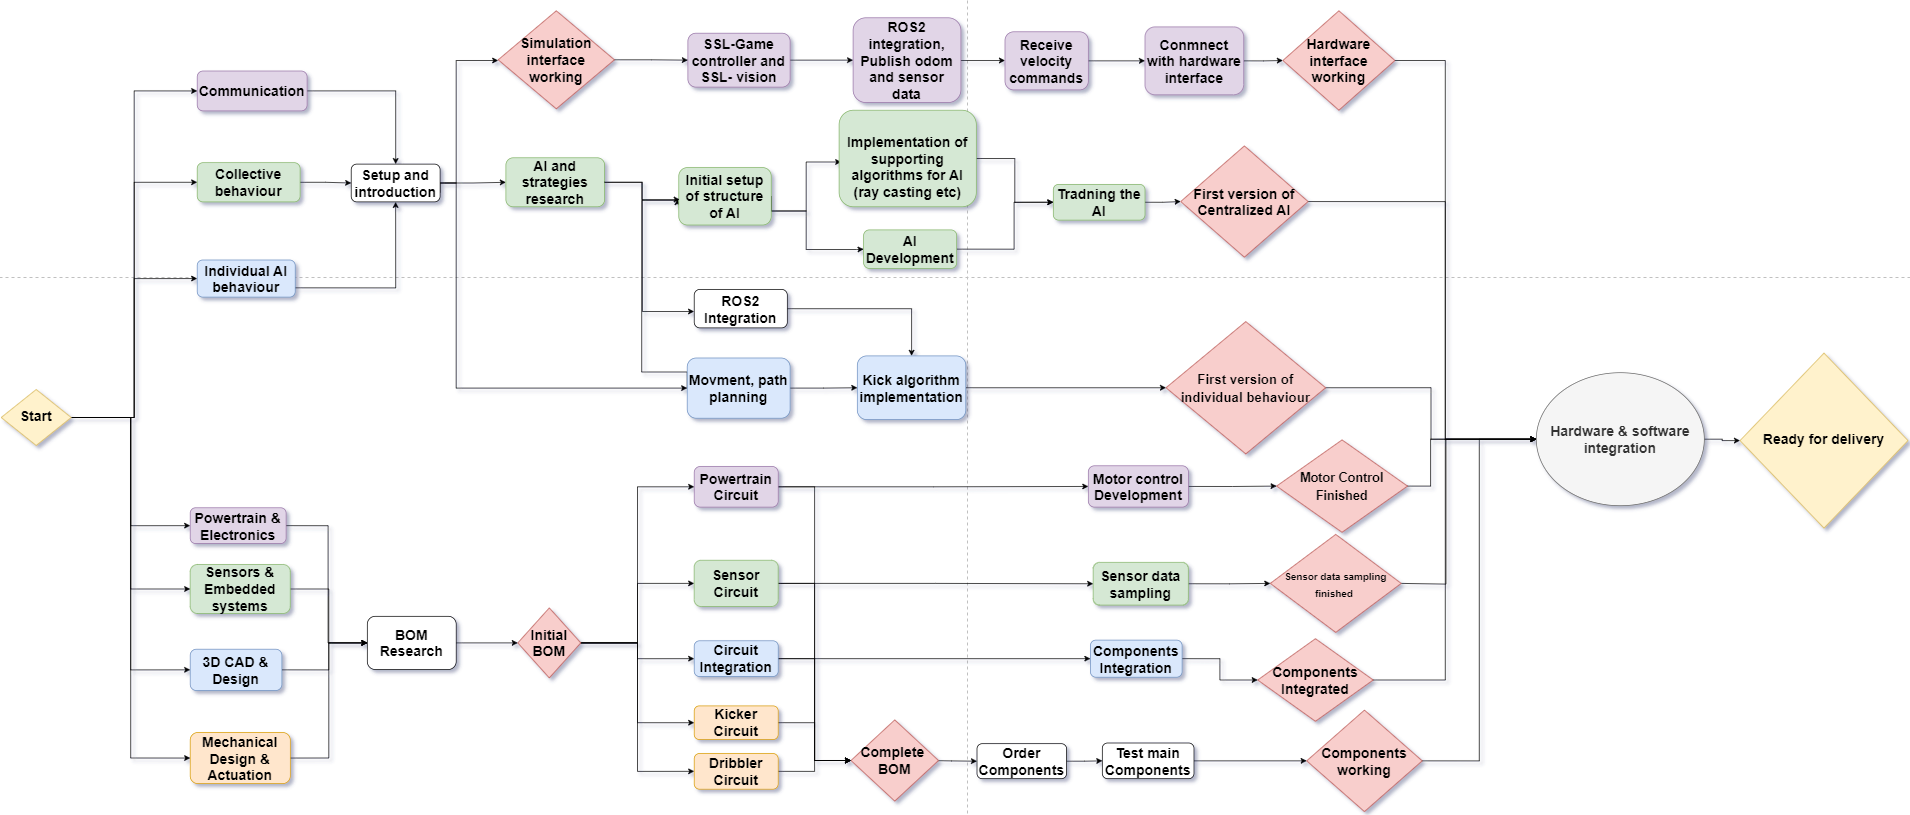
\includegraphics[width=\linewidth]{images/MileStone.png}
    \caption{The milestone plan for the project.}
    \label{fig:mile_stone} 
\end{sidewaysfigure}

%===============================================================================

\section{Appendix: Bill of Materials}
\label{appendix:bom}

\begin{table}[H]
    \centering
    \renewcommand{\arraystretch}{1.2} % Adjust row height
    \large % Increase text size
    \begin{tabularx}{\textwidth}{|X|X|X|X|} \hline
         \textbf{Component} & \textbf{Features} & \textbf{Purpose} & \textbf{Price (SEK)}  \\ \hline
         DF45L024048-A-Brushless \ac{dc} Motor & Good torque, built-in sensors, small footprint & Motors connected to the wheels to drive the robot in all directions & $3273.6\ (818.4 \times 4)$ \\ \hline
         Hobbywing FPV XRotor 3110 900KV & Supports very high \ac{rpm} needed for the dribbler & Part of the dribbler system that adds spin to the ball to increase control & $175.2$\\ \hline
         Aerostar 30A RVS G2 32bit \ac{esc} & PWM-based \ac{esc} to control motor speed & To control the motors & $736\ (147.2 \cdot4)$\\ \hline
         Arduino Nano & Samples output current of each phase, closed-loop PID system to regulate PWM signal & Regulate the PWM signal & $1196\ (299 \cdot4)$ \\ \hline
         Hall effect current sensor & Hall effect current sensor to measure the current of each phase in the \ac{esc} & Measure phase current &$576 (48\cdot4\cdot3)$\\ \hline
         ESP32-WROVER-IE & Low power consumption, Wi-Fi communication & A \ac{mcu} to collect sensory information, communicate with the external computer, and control the motors & Sponsored by \ac{mdu}\\ \hline
         Raspberry Pi 4 Model B/8GB & Multiple connection ports, 8GB \ac{ram}, low power mode & A \ac{mcu} to handle camera input, run Nav2, and send motor instructions to the ESP32 & $979$\\ \hline
         6s 1300mAh-120C-GNB HV XT60 & Sufficient energy capacity, low price, small footprint, low weight & Provide voltage and current to all sensors and actuators & $351.2$\\ \hline
         LT3750 & Capacitor charging controller for kicker, adjustable output voltage, integrated security control & Charges capacitors to sufficient levels (up to 300V) for passing and shooting & $146.9$\\ \hline
         iC-PX2604 and PX01S 26-30 & Optical encoder and wheel for accurate wheel orientation readings & Uses slits in the encoder wheel to read position & $897.6\ (224.4 \cdot4)$\\ \hline
         WSEN-ISDS 6 Axis \ac{imu} & Reads up to $\pm 16g$ and $\pm 2000$ \ac{dps} &  & Sponsored by Würth Electronics\\ \hline
         Raspberry Pi Camera Module 3 & Commonly used in \ac{ssl} modules for object detection &  & $369$\\ \hline
         LEDEX 195207-228 & Solenoid for the kicker &  & Sponsored by \ac{mdu}\\ \hline
    \end{tabularx}
    \caption{The preliminary \acl{bom} for the project.}
    \label{tab:bom}
\end{table}

%===============================================================================

\bibliographystyle{unsrtnat}
\bibliography{references}

% \printbibliography
% \appendices

\end{document}
%===============================================================================